\documentclass[12pt,a4paper]{article}
\usepackage[left=25mm,right=10mm,top=20mm,bottom=20mm,footskip=10mm]{geometry}
\usepackage{fontspec}
\setmainfont{Times New Roman}
\setsansfont{DejaVu Sans}[Scale=.88]
\setmonofont{DejaVu Sans Mono}[Scale=.78]
\usepackage{polyglossia}
\newfontfamily\cyrillicfont{Times New Roman}[Script=Default]
\setdefaultlanguage{russian}
\setotherlanguage{english}
\usepackage{amsmath,amssymb,graphicx,booktabs,tabularx,array,longtable}
% Scalable outlines already available locally, at the requested math size.
\DeclareFontFamily{OML}{cmm}{\skewchar\font127}
\DeclareFontShape{OML}{cmm}{m}{it}{<->cmmi10}{}
\DeclareFontShape{OT1}{cmr}{m}{n}{<->cmr10}{}
\usepackage{setspace,indentfirst,caption,titlesec,enumitem,xcolor,hyperref}
\definecolor{link}{HTML}{215B7B}
\hypersetup{unicode=true,colorlinks=true,linkcolor=black,citecolor=black,urlcolor=link,filecolor=link,
 pdfauthor={Нефедов Дмитрий Львович},pdftitle={Управление перевёрнутым маятником методами обучения с подкреплением},
 pdfsubject={Отчёт об исследовательском проекте}}
\onehalfspacing
\setlength{\parindent}{1.25cm}
\setlength{\parskip}{0pt}
\setlength{\emergencystretch}{5em}
\setlength{\textfloatsep}{12pt}
\setlength{\floatsep}{10pt}
\setlength{\intextsep}{10pt}
\clubpenalty=10000\widowpenalty=10000
\titleformat{\section}{\large\bfseries}{\thesection}{.6em}{}
\titleformat{\subsection}{\normalsize\bfseries}{\thesubsection}{.6em}{}
\titlespacing*{\section}{0pt}{12pt}{8pt}
\titlespacing*{\subsection}{0pt}{10pt}{4pt}
\captionsetup{font=small,labelsep=endash}
\captionsetup[figure]{name=Рисунок,justification=centering}
\captionsetup[table]{position=top,justification=raggedright,singlelinecheck=false}
\setlist{itemsep=0pt,topsep=3pt,parsep=0pt,leftmargin=1.25cm}
\newenvironment{smalltable}{\begin{singlespace}\fontsize{10}{12}\selectfont\setlength{\tabcolsep}{5pt}\renewcommand{\arraystretch}{1.15}}{\end{singlespace}}
\newcommand{\chapterstart}[1]{\clearpage\section{#1}}
\newcommand{\unnumbered}[1]{\clearpage\phantomsection\section*{#1}\addcontentsline{toc}{section}{#1}}
\makeatletter
\newcommand{\reportappendix}[2]{\unnumbered{Приложение #1. #2}\protected@edef\@currentlabel{#1}}
\makeatother
\newcommand{\source}[1]{\par\smallskip{\footnotesize\noindent Источник: #1\par}}
\newcommand{\fig}[4]{\begin{figure}[htbp]\centering\includegraphics[width=#3\linewidth]{figures/#1.pdf}\caption{#2}\label{#4}\end{figure}}
% One repository entry point; the PUBLIC repository is readable without authentication.
\newcommand{\SubmissionRepositoryURL}{https://github.com/nefedovdima/cartpole-coursework-submission}
% Keep source identities for integrity checks; print only descriptive labels.
\newcommand{\eref}[2]{#2}
\newcommand{\vref}[2]{#2}
\newcommand{\applink}[2]{#2}

\begin{document}
\begin{titlepage}
\centering
ПРАВИТЕЛЬСТВО РОССИЙСКОЙ ФЕДЕРАЦИИ\par
ФГАОУ ВО НАЦИОНАЛЬНЫЙ ИССЛЕДОВАТЕЛЬСКИЙ УНИВЕРСИТЕТ\par
«ВЫСШАЯ ШКОЛА ЭКОНОМИКИ»\par
\vspace{7mm}
Факультет компьютерных наук\par
Образовательная программа\par
«Прикладная математика и информатика»\par
\vspace{25mm}
Отчёт об исследовательском проекте на тему:\par
\vspace{5mm}
{\large\bfseries Управление перевёрнутым маятником\par
методами обучения с подкреплением\par}
\vspace{24mm}
\hfill\begin{minipage}{.58\linewidth}
Выполнил:\\студент группы БПМИ-233\\Нефедов Дмитрий Львович\par
\vspace{8mm}
Руководитель проекта:\\Бондарев Андрей Олегович\\
Эксперт Проектно-учебной\\лаборатории робототехники\\
Факультет компьютерных наук НИУ ВШЭ
\end{minipage}
\vfill Москва, 2026
\end{titlepage}
\setcounter{page}{2}
{\singlespacing\small\tableofcontents}
\unnumbered{Аннотация}
Исследуется подъём маятника на тележке из нижней области и его последующее удержание сверху при ограничениях движения. В идеализированной модели с управляемым ускорением тележки сравниваются четыре алгоритма обучения с подкреплением и классический траекторный регулятор. Защитный фильтр проверяет запрос контроллера и при необходимости меняет ускорение, чтобы сохранить тормозной запас тележки. Успех удержания и соблюдение ограничений оцениваются отдельно.

Исследованы 33 обучения по 100\,000 переходов: основная серия, ограниченный подбор настроек и их проверка на новых реализациях случайности. Два из изученных методов с фильтром решают все двадцать проверочных сценариев в трёх исходных обучениях. Увеличенный начальный сбор опыта улучшает результат отбора двух неуспешных процедур, но не проходит заранее установленный критерий подтверждения на новых обучениях. Показан случай роста суммарной награды при ухудшении удержания из-за скорости тележки.

Отдельно семь закреплённых контроллеров испытаны на 140 общих стартовых состояниях: 1960 эпизодов, 980 пар с фильтром и без него. Число успехов увеличивается с 441/980 до 796/980; наблюдённые превышения желаемой границы с допуском исчезают. Однако 184/980 эпизода с фильтром не выполняют заключительное удержание, хотя достигают горизонта. Выводы относятся к фиксированному диагностическому набору и симуляции. Независимая итоговая оценка и аппаратные испытания не проводились.

\medskip\noindent\textbf{Ключевые слова:} перевёрнутый маятник; обучение с подкреплением; управление с ограничениями; защитный фильтр; повторяемость обучения; начальные условия; вычислительный эксперимент.

\unnumbered{Введение}
Перевёрнутый маятник на тележке представляет собой простую по устройству, но содержательную задачу управления. Привод перемещает тележку, а маятник вращается свободно: отдельного управляющего воздействия на его оси нет. Для подъёма из нижнего положения нужно передать маятнику энергию движением шарнира. Вблизи верхнего неустойчивого равновесия задача меняется: необходимо погасить угловую скорость и компенсировать отклонения. Ограниченная длина направляющей связывает эти этапы. Движение, полезное для подъёма, может не оставить тележке места для торможения.

При известной модели эту задачу можно решать с помощью планирования траектории и обратной связи. Альтернативу даёт обучение с подкреплением: управляющая программа улучшает поведение по опыту взаимодействия со средой. Существование обоих подходов делает маятник удобным объектом сравнительного исследования. Практический вопрос состоит не только в том, способен ли алгоритм однажды поднять маятник, но и в том, повторяется ли результат обучения, сохраняется ли он при других стартах и соблюдаются ли ограничения движения.

\textbf{Цель работы} — исследовать качество подъёма и удержания перевёрнутого маятника классическим регулятором и выбранными методами обучения с подкреплением в общей модели с ограничениями. Объект исследования — система «тележка — маятник» с управляемым ускорением тележки. Предмет исследования — результативность управления, повторяемость обучения и чувствительность закреплённых контроллеров к начальным условиям и защитному фильтру.

Для достижения цели решаются следующие задачи:
\begin{enumerate}
\item согласовать модель, ограничения, наблюдение агента и физический критерий успешного удержания;
\item организовать сравнение DQN, DDPG, SAC, TQC и классического траекторного регулятора при явно заданных условиях;
\item проверить ограниченный подбор настроек и повторяемость выбранного улучшения на новых запусках обучения;
\item оценить одни и те же контроллеры на структурированном наборе начальных состояний с фильтром и без него;
\item разделить причины неуспеха по наблюдаемым признакам и установить границы выводов.
\end{enumerate}

В обучении с подкреплением (reinforcement learning, RL) \emph{агент} получает наблюдение и выбирает действие. Правило такого выбора называется \emph{политикой}. Среда исполняет действие и возвращает новое наблюдение и численную \emph{награду}. Одна попытка управления до заданного времени или досрочной остановки называется \emph{эпизодом}. Агент обучается увеличивать накопленную награду, однако её рост не обязательно означает выполнение физической задачи. Поэтому награда, успех удержания и соблюдение ограничений в работе измеряются раздельно.

Случайная инициализация нейросетей и сбор опыта влияют на найденную политику. Начальное значение генераторов случайных чисел (\emph{seed}) задаёт конкретную реализацию случайности. Разные seed обучения не означают разные границы распределения начальных состояний. Сохранённые параметры модели образуют \emph{контрольную точку} (checkpoint). В работе различаются лучшая по правилу отбора точка и последние веса одного обучения; это две версии одной модели, а не два независимых запуска.

Для выбора модели используется \emph{валидация}: оценка на фиксированных состояниях, результаты которой участвуют в отборе. Такие состояния нельзя затем считать независимым итоговым тестом. Аналогично, проверка выбранной настройки на новых seed характеризует повторяемость обучения, но не заменяет испытание на новых физических стартах. Под \emph{робастностью} далее понимается эмпирическое сохранение качества при изменении начальных условий. Устойчивость к шумам, задержкам и ошибкам параметров в этот эксперимент не входит.

Защитный фильтр проверяет запрос контроллера и при необходимости меняет ускорение, сохраняя тормозной запас тележки. При включённом фильтре оценивается система «контроллер вместе с фильтром»: её успех нельзя целиком приписывать нейросети. В то же время защита положения не обеспечивает подъём и удержание сама по себе. Именно поэтому сравнение проводится как между процедурами обучения, так и между двумя режимами исполнения одних весов.

Эксперименты включают основную серию из 15 обучений, этап подбора настроек из 12 обучений и проверку выбранных настроек из шести обучений. Каждый запуск содержит 100\,000 переходов, суммарно — 3,3 млн. Дополнительно семь фиксированных контроллеров оценены на 140 общих стартовых состояниях: 1960 эпизодов, образующих 980 пар с фильтром и без него. Повторное использование стартов обеспечивает сопоставимость, но не превращает эти пары в независимую выборку из всего пространства состояний.

\textbf{Основные результаты.} SAC и TQC с фильтром решают все двадцать валидационных сценариев в каждом из трёх исходных обучений. Подбор увеличенного начального сбора опыта для DDPG с фильтром и SAC без него улучшает результат отбора, но не проходит последующую проверку повторяемости. В структурированной матрице включение фильтра увеличивает число успехов с 441/980 до 796/980 и устраняет наблюдённые превышения желаемой границы с учётом допуска. При этом 184/980 эпизода с фильтром завершают горизонт без успешного заключительного удержания. Эти результаты показывают различие между допустимым движением тележки и выполнением полной задачи.

\textbf{Вклад проекта} состоит в построении согласованной экспериментальной цепочки на основе лабораторного симулятора и в сравнительном анализе полученных результатов. Подготовлены интерфейс среды, обработка событий ограничений, защитный слой, протокол выбора моделей и средства анализа. Разделены влияние фильтра, случайности обучения и начального состояния; сохранены отрицательные результаты. Лабораторная динамика, основа классического управления и библиотечные алгоритмы обучения имеют самостоятельное происхождение. Разработка нового универсального алгоритма управления не заявляется.

Работа ограничена симуляцией с идеально задаваемым ускорением. Обученные политики на оборудовании не испытывались, независимая итоговая оценка после всех решений разработки не проводилась. Эти ограничения учитываются при обсуждении каждого результата.


\chapterstart{Связанные работы и выбор подходов}
\label{sec:review}
Рассматриваемая задача объединяет три вопроса: как построить управляющий закон, как соблюсти ограничения и как корректно сравнить результаты. Литература по каждому из них даёт свои основания для экспериментального протокола. Ниже обсуждается не общий рейтинг алгоритмов, а то, какие свойства подходов существенны именно для подъёма маятника на короткой направляющей.

\subsection{Классическое управление как содержательная база сравнения}
Линейно-квадратичный регулятор (Linear Quadratic Regulator, LQR) выбирает линейную обратную связь по отклонению от равновесия, а его коэффициенты определяются из квадратичного штрафа за отклонение состояния и за усилие управления. Для нелинейного маятника такой регулятор применяют к линеаризации около верхнего положения: он решает задачу локальной стабилизации и сам по себе подъёма снизу не задаёт. Дополняет его траекторная оптимизация — сначала строится номинальное движение, затем регулятор компенсирует отклонения от него. Оба метода изложены Р.~Тедрейком~\cite{tedrake_lqr,tedrake_traj}.

Разделение подъёма и стабилизации вытекает из нелинейности задачи. Линеаризация описывает малые отклонения от выбранного движения, и её точность не распространяется автоматически на нижнее положение маятника, поэтому траекторный регулятор использует изменяющееся во времени опорное движение, а стационарный LQR предназначен для локальной стабилизации около верхнего равновесия. В реализованном здесь контроллере переключение на него выполняется по окончании запланированной траектории, то есть по времени, а не по проверке близости состояния к равновесию. Сопоставлять такой подход с обучаемой политикой нужно по полной задаче подъёма и удержания, сохраняя при этом сведения о том, как построена опорная траектория.

В проекте классическая процедура включает заранее сохранённую траекторию подъёма, слежение с обратной связью и переход к LQR. Она нужна не только как техническая проверка симулятора: если известная модель уже допускает эффективное классическое решение, успех обучаемого метода следует сопоставлять именно с ним, а не только с бездействием. Одна фиксированная траектория, впрочем, не обязана подходить всем расширенным стартам, и это учитывается при интерпретации результатов Главы~\ref{sec:robust}.

Исходный лабораторный проект \texttt{robotics-laboratory/cart-pole} предоставляет модель и основу классического управления~\cite{laboratory}. Его вход — ускорение тележки, а не сила двигателя, и уже поэтому совпадение названия CartPole с другими средами не делает результаты сопоставимыми: проверять нужно уравнения, начальную область, длину направляющей и критерий успеха. Настоящая работа сохраняет лабораторную динамику и строит вокруг неё общий экспериментальный протокол.

\subsection{Четыре подхода к обучению управляющего закона}
Все рассматриваемые методы опираются на нейросетевую оценку ценности действия — ожидаемой будущей суммы наград при его выборе и последующем поведении. Такая оценка позволяет учитывать отложенный результат: кратковременное движение тележки от центра может оказаться полезным, если впоследствии оно позволяет поднять маятник. Ценность не равна немедленной награде и сама является приближением, которое меняется по ходу обучения.

\textbf{DQN} (Deep Q-Network) обучает оценки для дискретного набора действий. Повторное использование переходов из буфера опыта и медленно меняющаяся целевая сеть снижают зависимость обучения от последовательности соседних наблюдений~\cite{mnih}. В нашей задаче DQN выбирает один из девяти запросов ускорения — это простой дискретный подход, но набор доступных ему запросов заведомо уже, чем у непрерывных методов. Общая физическая среда, как видно уже здесь, не означает одинакового класса возможных управляющих законов.

\textbf{DDPG} (Deep Deterministic Policy Gradient) предназначен для непрерывных действий. Сеть управления, \emph{актор} (actor), выдаёт действие, а сеть оценки, \emph{критик} (critic), предсказывает его ценность; актор меняется в направлении роста предсказанной ценности, а исследование обеспечивается добавленным шумом~\cite{lillicrap}. DDPG выбран как базовый непрерывный метод. Его зависимость от качества критика делает особенно полезной проверку разных seed, хотя сама по себе архитектура ещё не объясняет неуспех конкретного обучения.

\textbf{SAC} (Soft Actor-Critic) сочетает рост ожидаемого возврата с энтропией — мерой разнообразия распределения действий. Стохастическая политика поддерживает исследование, а две оценки критиков используются для более осторожной цели обновления~\cite{haarnoja_sac}; вариант с автоматической настройкой веса энтропии описан в развитии метода~\cite{haarnoja_apps}. Для маятника SAC интересен как способ находить последовательность подъёма без заранее заданной траектории. Энтропия при этом остаётся свойством распределения действий и ограничением на положение тележки не является, так что заменить защиту она не может.

\textbf{TQC} (Truncated Quantile Critics) сохраняет энтропийного актора, но критики предсказывают квантили распределения возврата вместо одного среднего, и при построении обучающей цели часть наиболее высоких прогнозов отбрасывается~\cite{kuznetsov}. Это механизм контроля переоценивания, а не встроенная проверка физических границ. Сопоставление SAC и TQC показывает результат двух полных процедур; без отдельного эксперимента с выключенным усечением оно не устанавливает, что возможное преимущество вызвано именно квантилями.

Четыре метода вместе покрывают несколько разных способов построения политики: дискретный выбор запросов, детерминированное непрерывное управление, стохастическое управление с энтропийным критерием и его развитие с распределительной оценкой возврата. Исчерпывающим обзором современных алгоритмов такой набор, конечно, не является — он выбран для содержательного сравнения при доступном бюджете. Добавление новых методов без сопоставимого подбора параметров само по себе не сделало бы выводы сильнее.

Различия алгоритмов не следует путать с доказанными причинами экспериментальных исходов, и дальше это правило применяется последовательно. Успешность TQC не доказывает пользу усечения квантилей, пока нет сравнения с отключённым усечением. Неудача DQN не устанавливает, что девяти действий недостаточно: одновременно влияют обучение оценки ценности, исследование среды и бюджет переходов. Поэтому результаты интерпретируются на уровне полных процедур; об отдельных механизмах эти данные не говорят.

Использованы реализации Stable-Baselines3 и SB3-Contrib~\cite{raffin,contrib}: библиотечные алгоритмы не переписывались и авторскими здесь не выдаются, а разработанная часть проекта описана в Главе~\ref{sec:design}. Общие небольшие сети и одинаковый бюджет взаимодействий делают сравнение обозримым, но индивидуально оптимальных настроек каждому методу не гарантируют. Выводить из полученного порядка результатов общий рейтинг алгоритмов на всех задачах управления было бы ошибкой.

\subsection{Защитный фильтр и достоверность сравнения}
Предиктивные защитные фильтры отделяют предложение контроллера от проверки его допустимости. У Wabersich и Zeilinger фильтр использует прогноз ограниченной нелинейной системы и при необходимости корректирует вход~\cite{wabersich}. В нашем случае реализована существенно более узкая процедура — аналитический прогноз координаты и скорости тележки при постоянном ускорении. Воспроизведением общего нелинейного алгоритма из этой статьи она не является и гарантий для неопределённой динамики автоматически не наследует.

Safe-control-gym объединяет оценку качества и безопасности классических и обучаемых регуляторов, в том числе при возмущениях~\cite{yuan}. Для настоящей работы важен оттуда принцип раздельных метрик: агент может достичь цели, нарушив ограничение, либо сохранить ограничение, не достигнув цели. Шумы, задержки и ошибки параметров в нашем протоколе не испытывались, поэтому численные результаты здесь с этим набором задач напрямую не сопоставляются — он служит методологическим ориентиром.

Henderson и соавторы показывают, насколько выводы о глубоком обучении с подкреплением зависят от случайности и деталей процедуры~\cite{henderson}. Отсюда прямо следуют три решения протокола: сохранять каждый запуск, оценивать последние веса отдельно от лучших и проверять выбранную настройку на новых seed. Три значения seed не дают точной оценки распределения качества будущих обучений, но позволяют увидеть крупную неоднородность, которую единственный успешный пример скрыл бы полностью.

\subsection{Позиционирование настоящего исследования}
Из рассмотренных работ следуют три требования к сравнению: определить модель и критерии явно, поскольку одинаковое название задачи не гарантирует одинаковой динамики; измерять соблюдение ограничений отдельным механизмом и отдельными показателями, поскольку высокая награда сертификатом безопасности не является; и не считать результат единственного обучения оценкой повторяемости процедуры.

Настоящий проект реализует эти требования в лабораторной модели с ускорительным входом. Его результат — не универсальное преимущество обучения с подкреплением над классическим управлением, а воспроизводимое сопоставление конкретных процедур вместе с диагностикой их ограничений. Общая модель делает физические результаты сравнимыми, а разделение отбора, новых запусков и новых стартов позволяет каждый раз сказать, на какие именно данные опирается вывод. В следующей главе эти принципы переводятся в уравнения и измеряемые критерии.

\chapterstart{Модель, защитный фильтр и критерии качества}
\label{sec:model}
\subsection{От установки к расчётной модели}
Тележка перемещает шарнир маятника вдоль горизонтальной направляющей. Движение шарнира меняет угол маятника, хотя отдельного привода на его оси в расчётной модели нет. Рисунок~\ref{fig:stand_photo} показывает лабораторную установку из предоставленной видеозаписи, а Рисунок~\ref{fig:stand_illustration} помогает различить основные узлы. Оба изображения объясняют устройство стенда и не свидетельствуют об испытании наших обученных политик на нём.
\begin{figure}[htbp]
\centering
\begin{minipage}[t]{.47\linewidth}\centering
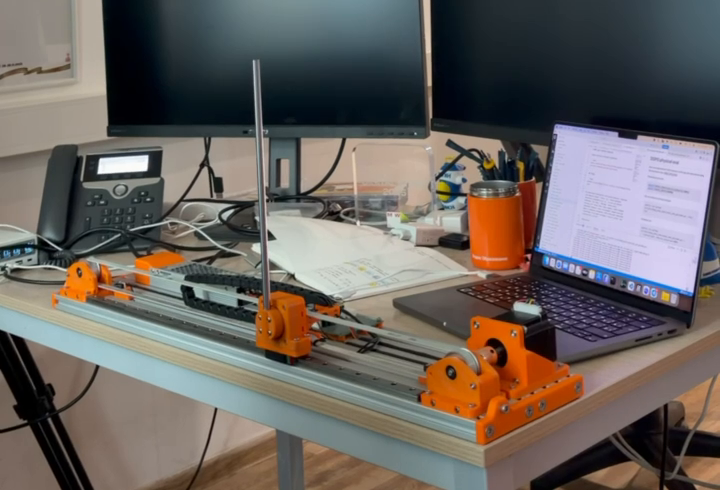
\includegraphics[width=\linewidth]{figures/laboratory_stand_photo.png}
\caption{Лабораторная установка.}\label{fig:stand_photo}
\end{minipage}\hfill
\begin{minipage}[t]{.49\linewidth}\centering
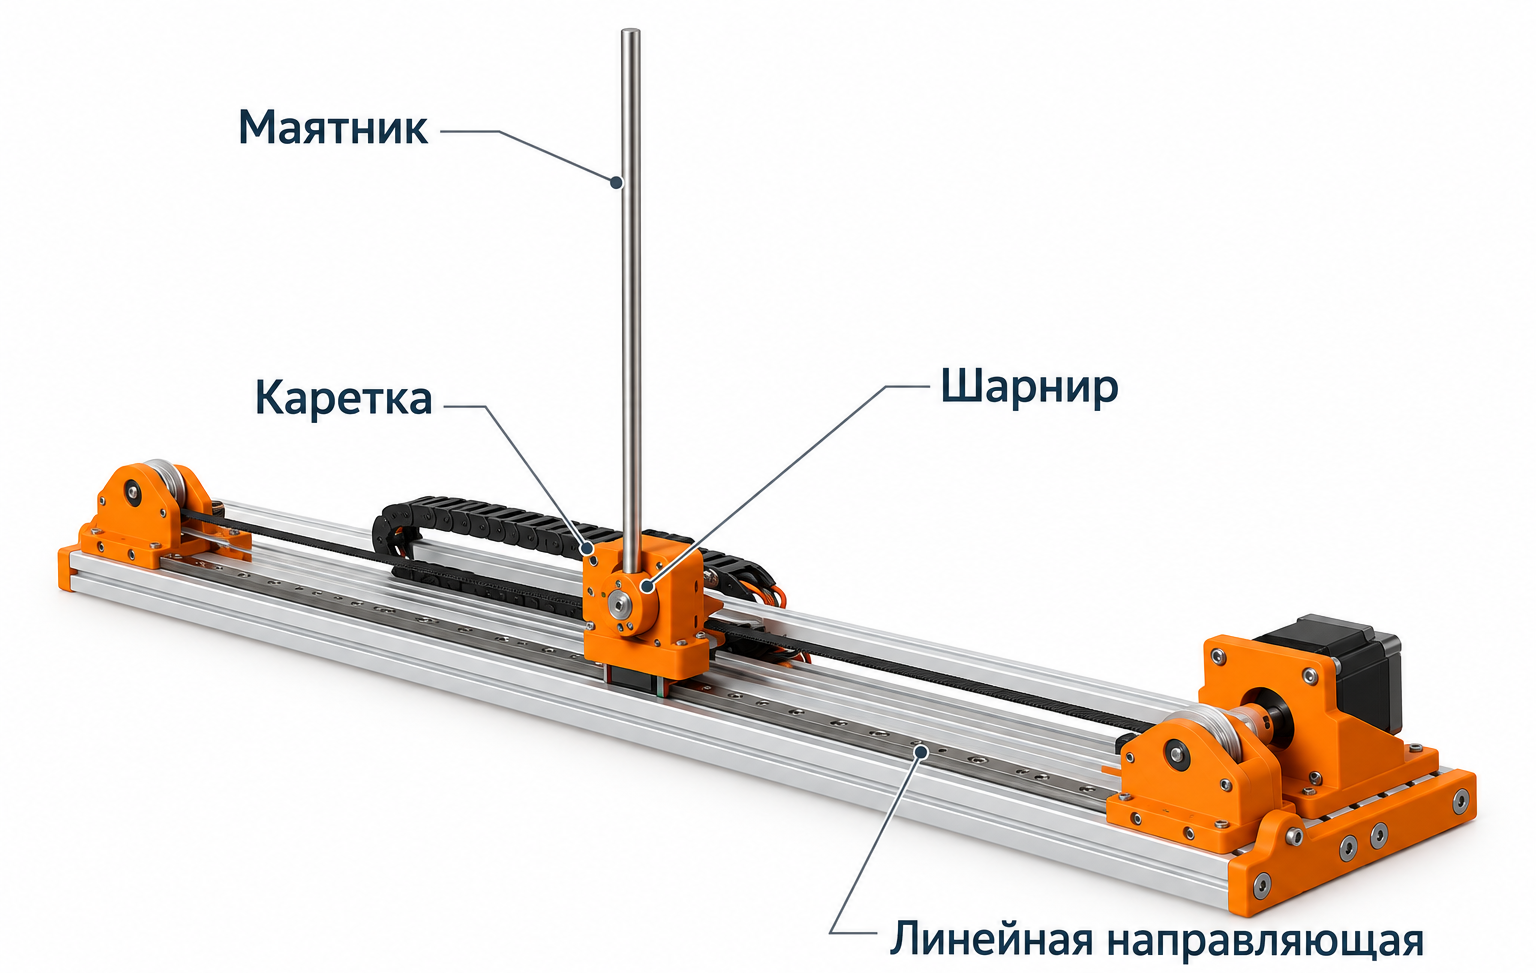
\includegraphics[width=\linewidth]{figures/laboratory_stand_annotated.png}
\caption{Основные узлы установки. Схематическое изображение.}\label{fig:stand_illustration}
\end{minipage}
\end{figure}

Состояние обозначим $s=(x,v,\theta,\omega)$. Здесь $x$ — горизонтальная координата шарнира в метрах, $v=\dot x$ — скорость тележки в м/с, $\theta$ — угол в радианах от вертикали вниз, $\omega=\dot\theta$ — угловая скорость в рад/с. Положительное направление $x$ — вправо, и при небольшом положительном $\theta$ конец маятника смещён вправо от нижней вертикали. Нижнему равновесию соответствует $\theta=0$, верхнему — $\theta=\pi$ с точностью до полного оборота $2\pi$.

Рисунок~\ref{fig:model} закрепляет геометрические соглашения. В классическом регуляторе используется другой порядок компонент, $q=(x,\theta,v,\omega)$, — это перестановка того же физического состояния, а не иная модель.
\begin{figure}[htbp]\centering
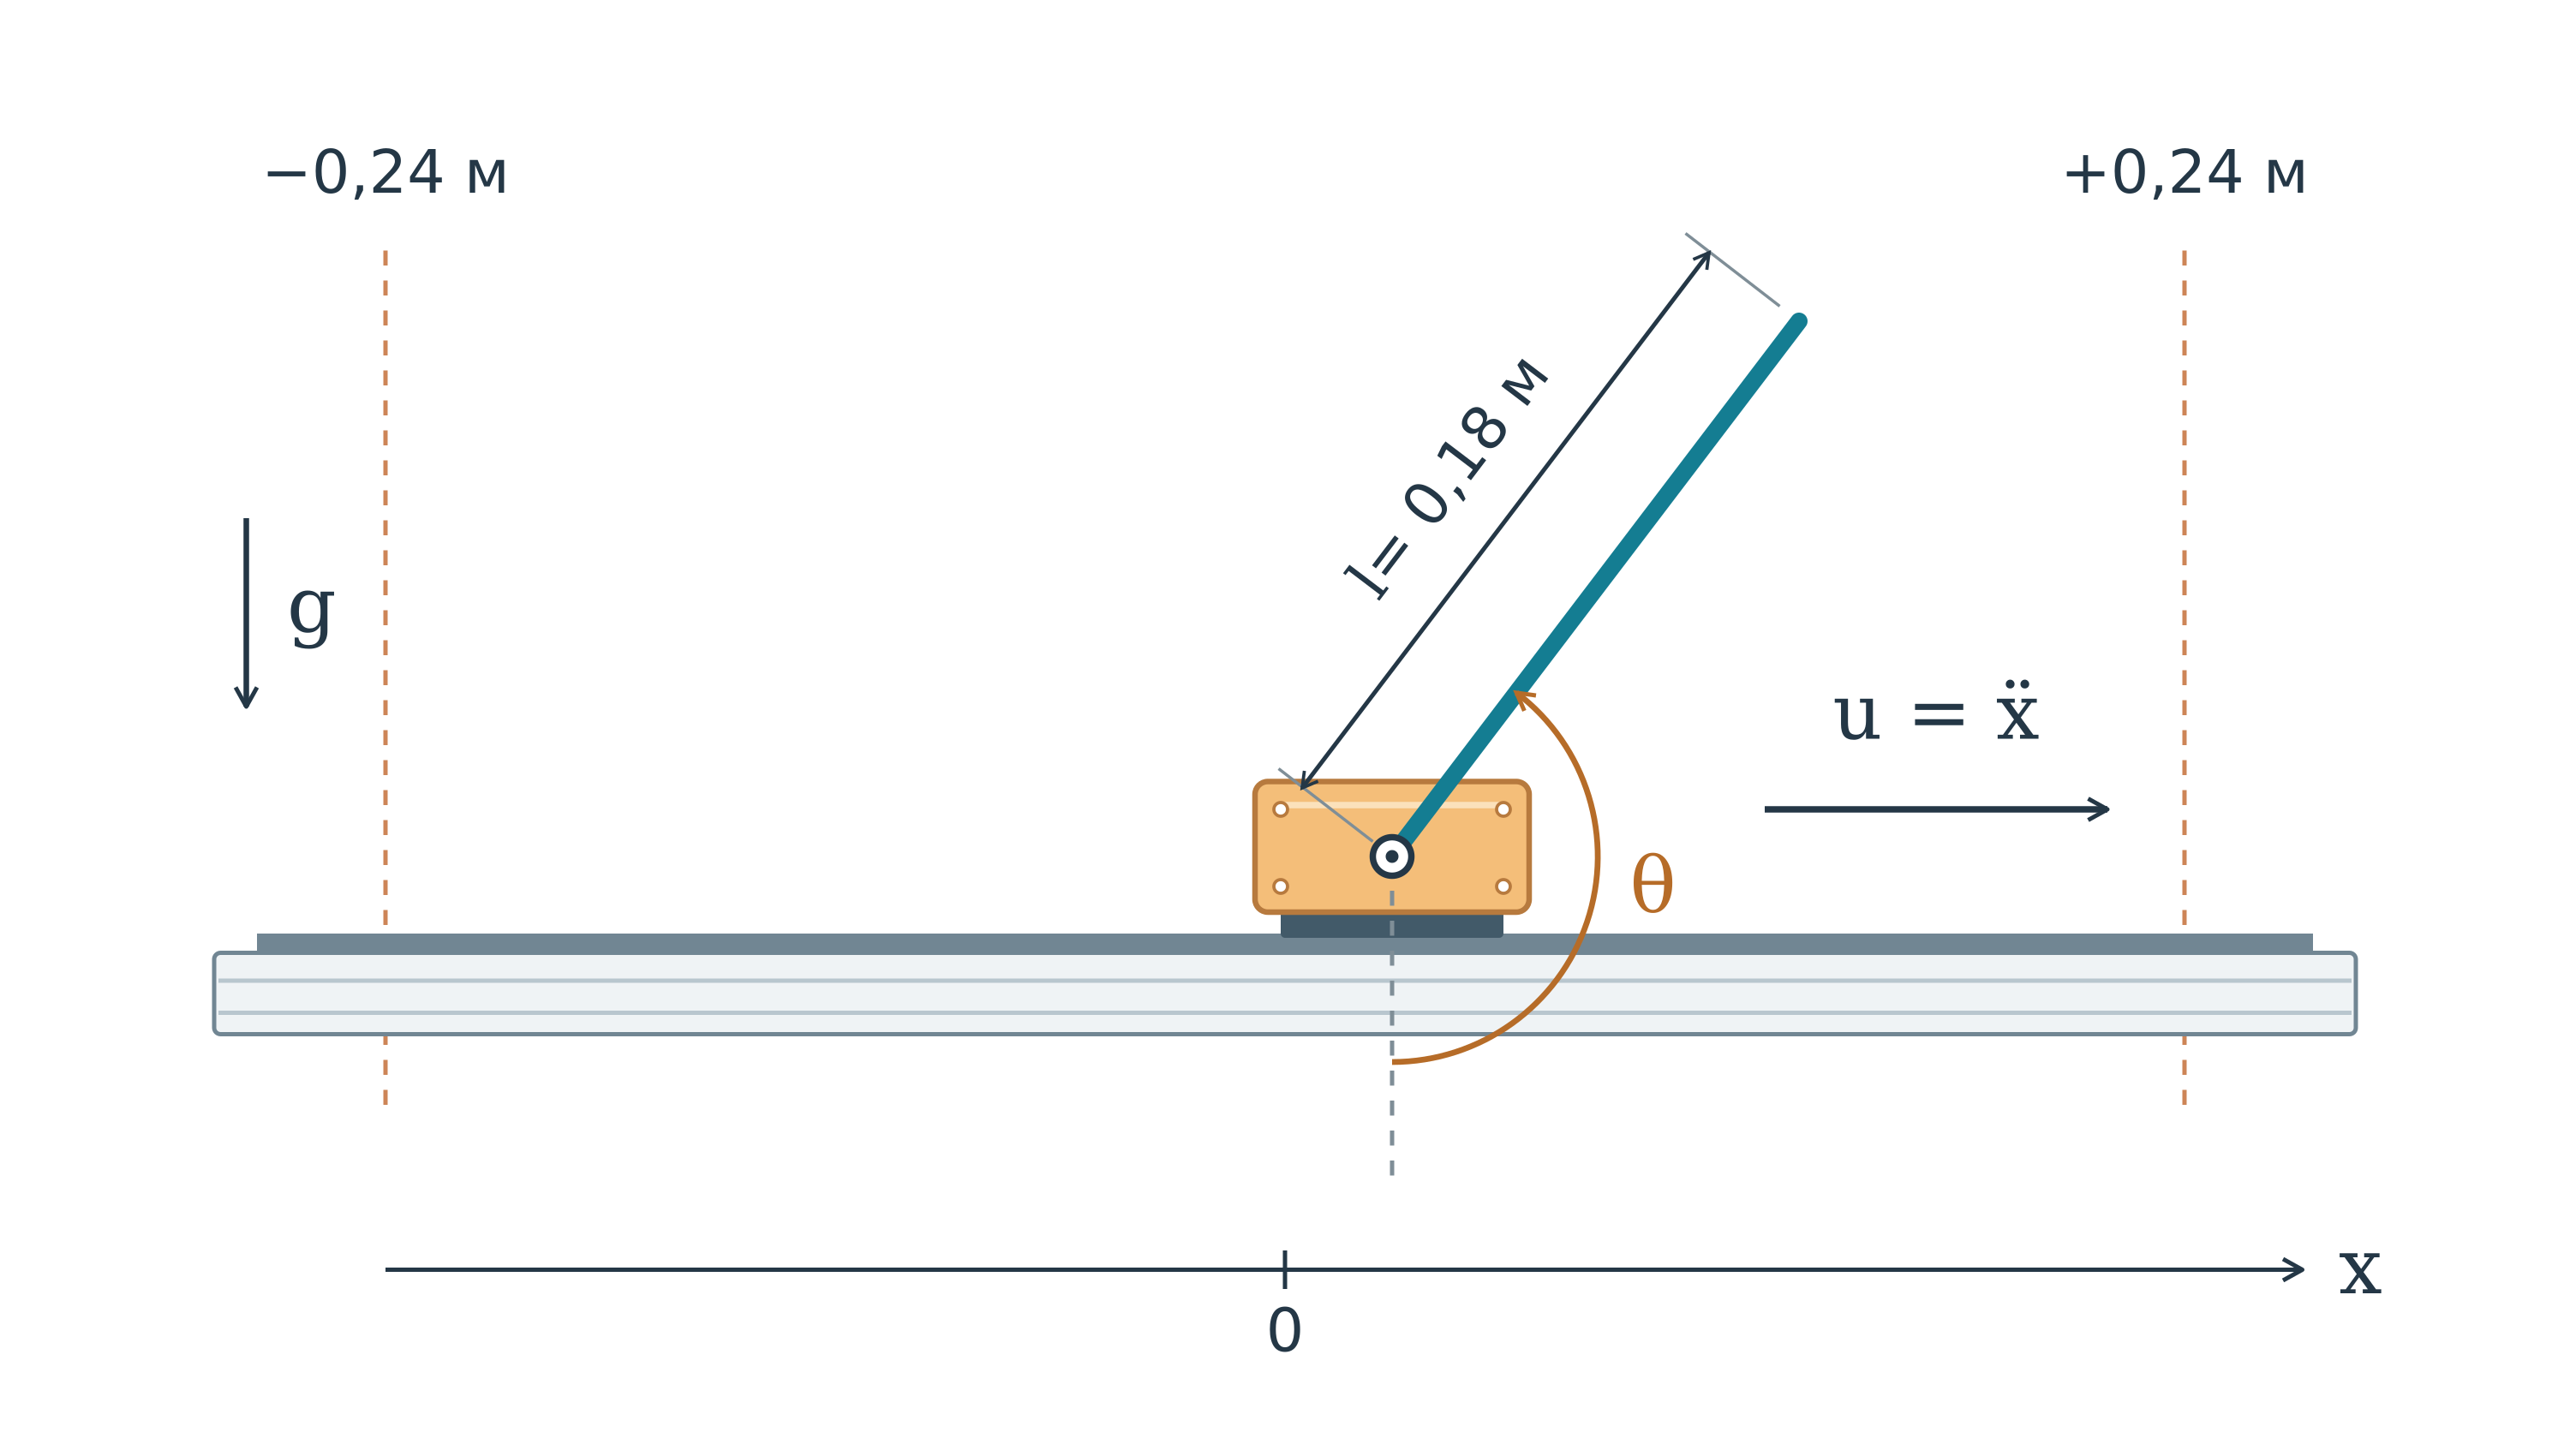
\includegraphics[width=.93\linewidth]{figures/cartpole_model_scheme.png}
\caption{Соглашения расчётной модели: угол от нижней вертикали, вход $u=\ddot x$, длина $l=0{,}18$ м. Пунктир — желаемые границы положения шарнира $\pm0{,}24$ м.}\label{fig:model}
\end{figure}

\subsection{Уравнения и постоянное управление между отсчётами}
Контроллер задаёт ускорение тележки $u$ в м/с$^2$. Приняты уравнения
\begin{equation}
\dot x=v,\qquad \dot v=u,\qquad \dot\theta=\omega,\qquad
\dot\omega=-\frac{u\cos\theta+g\sin\theta}{l}.
\label{eq:physics}
\end{equation}
Положение конца идеализированного маятника относительно шарнира равно $(l\sin\theta,-l\cos\theta)$, а проекция ускорения на касательную даёт $l\ddot\theta+u\cos\theta=-g\sin\theta$, что согласуется с последним уравнением~\eqref{eq:physics}. Около верха, положив $\varphi=\theta-\pi$, получаем $\ddot\varphi\approx(g/l)\varphi+u/l$: малое отклонение нарастает экспоненциально, и без подходящей обратной связи маятник падает.

Управляемое ускорение — свойство лабораторной модели, унаследованное вместе с ней, и оно заметно упрощает постановку. Реакция маятника не изменяет предписанное ускорение тележки, а масса в уравнения вообще не входит. Не описаны и трение, инерция и насыщение привода по силе, люфт, шум измерений и задержки. Отсюда следует практический вывод: найденное управление нельзя перенести на установку одним пересчётом единиц — понадобится отдельно проверить и исполнение ускорения, и адекватность самой динамики.

Параметры приведены в Таблице~\ref{tab:physics}. Длина и рабочие пределы восходят к лабораторной конфигурации и в экспериментальном контракте заданы явно вместе с $g$ и аварийными пределами. Это настройки симуляции, а не результаты идентификации оборудования. Копии контракта и конфигураций перечислены в Приложении~\ref{app:repro}.
\begin{table}[htbp]\caption{Параметры модели и уровни ограничений}\label{tab:physics}
\begin{smalltable}\begin{tabularx}{\linewidth}{@{}l l X@{}}\toprule
Величина & Значение & Смысл\\\midrule
$g$, $l$ & $9{,}8$ м/с$^2$; $0{,}18$ м & Ускорение тяжести и длина маятника\\
$\Delta t$, $T$ & $0{,}01$ с; $10$ с & Интервал управления и горизонт эпизода\\
$A$ & $4$ м/с$^2$ & Максимум приложенного $|u|$ при обоих режимах\\
$X$, $V$ & $0{,}25$ м; $2$ м/с & Границы прекращения эпизода по $x,v$\\
$L_{\rm desired}$ & $0{,}24$ м & Желаемая граница защиты по положению\\
Аварийный $|x|$ & $0{,}27$ м & Дополнительный предел исходного симулятора\\
Аварийные $|v|$, $|u|$ & $2{,}5$ м/с; $5$ м/с$^2$ & Внутренняя аварийная политика\\
Интегратор & Адаптивный RK3 & Точность $10^{-6}$, шаг не более $0{,}01$ с; фиксированный шаг выключен\\\bottomrule
\end{tabularx}\end{smalltable}\end{table}

Между моментами управления команда постоянна, поэтому за интервал длины $h$ движение тележки известно аналитически:
\begin{equation}
x(\tau)=x_0+v_0\tau+\tfrac12u\tau^2,\qquad
v(\tau)=v_0+u\tau,\qquad 0\leq\tau\leq h.
\label{eq:cart}
\end{equation}
Формулы~\eqref{eq:cart} позволяют проверить весь интервал целиком, включая внутренний экстремум $x$, а не только конечный отсчёт. Общий исполнитель команд находит первое предстоящее нарушение $|x|\leq X$ или $|v|\leq V$ и останавливает переход ровно на границе, причём касание с возвращением внутрь выходом не считается. Состояние маятника до фактического момента остановки вычисляет исходный Drake — упрощённый аналитический интегратор тележки его не подменяет.

Событие достижения границы положения означает, что эпизод остановлен перед выходом за $\pm0{,}25$ м. Численного превышения этого предела оно не подразумевает и отличается от превышения желаемых $\pm0{,}24$ м, о котором речь пойдёт ниже. Переход при этом может оказаться укороченным или нулевым, если из граничного состояния движение направлено наружу. После терминального события следующее исполнение запрещено до нового сброса среды, а ошибки симулятора и исключения интегратора в успешное завершение не превращаются.

\subsection{Наблюдение, запрос и фактически приложенное ускорение}
Агенту передаётся не внутренний вектор Drake, а наблюдение
\begin{equation}
o(s)=\left(x/0{,}25,\ v/2,\ \sin\theta,\ \cos\theta,\ \omega/\sqrt{g/l}\right).
\label{eq:obs}
\end{equation}
Все величины в~\eqref{eq:obs} безразмерны: каждая координата поделена на свой характерный масштаб. Синус и косинус представляют угол без разрыва на границе полного оборота — две записи угла, отличающиеся на $2\pi$, описывают одну конфигурацию и дают одинаковое наблюдение. Само наблюдение округляется до \texttt{float32}, тогда как физический журнал хранит полный угол и исходные компоненты состояния. Классический регулятор наблюдения не использует и получает состояние непосредственно.

SAC, TQC и DDPG формируют нормированный запрос $a\in[-1,1]$, которому соответствует $u_{\rm req}=4a$. Для DDPG при обучении сначала добавляется исследовательский шум, а затем запрос ограничивается указанным диапазоном. DQN выбирает индекс одного из девяти ускорений $\{-4,-3,\ldots,3,4\}$ м/с$^2$ — равномерная сетка с шагом 1 м/с$^2$ по всему допустимому диапазону, включающая нуль. После фильтра исполняемая команда DQN может оказаться и между узлами этой сетки. Классическая обратная связь выдаёт физический запрос $u_{\rm req}$, который до общего исполнительного слоя может превышать $\pm4$.

Дальше запрос проходит через один из двух режимов. В режиме \emph{off} исполнитель просто ограничивает амплитуду: $u_{\rm cmd}=\min(A,\max(-A,u_{\rm req}))$. В режиме \emph{on} фильтр получает \textbf{исходный физический запрос}, а ограничение амплитуды входит в вычисляемое им множество допустимых команд. Величина вмешательства измеряется относительно исходного запроса и поэтому включает в себя и коррекцию амплитуды, если запрос выходил за пределы допустимых ускорений. Рисунок~\ref{fig:path} показывает весь путь команды.
\fig{command_path}{Путь команды и обратной связи. On — фильтр с ограничением амплитуды; off — обычный ограничитель. Оба режима сохраняют события рабочих границ. В буфер опыта поступает запрос агента, а в журнал — запрос, выбранная команда и фактическое исполнение.}{.96}{fig:path}

Точность здесь важна в обе стороны. Фильтр читает исходные $x,v$ полной точности, а не восстанавливает их из округлённого наблюдения; выбранное ускорение передаётся в Drake непосредственно, без повторной нормализации и обратного преобразования в \texttt{float32}. \emph{Приложенным ускорением} называется команда последнего реально выполненного перехода. Если время не продвинулось, приложенной команды нет: она считается отсутствующей, а не равной нулю, и эта оговорка существенна для отказа, случившегося до начала движения.

Буфер опыта (replay buffer) — хранилище прошлых переходов, из которого обучение многократно берёт примеры, — сохраняет наблюдение, \textbf{запрошенное} действие, награду, следующее наблюдение и признак окончания. В режиме on агент тем самым учится выбирать запросы к среде, которая уже включает защитное преобразование $F(s,u_{\rm req})$. Замена запроса исполненным ускорением изменила бы решаемую задачу, поэтому она не производится. Энтропия SAC и TQC тоже относится к запросам, а не к командам: несколько разных запросов могут после защиты дать одну и ту же команду.

\subsection{Почему одной проверки положения недостаточно}
Проверять текущую координату тележки мало, и это видно на числовом примере. Пусть тележка ещё внутри направляющей, но быстро движется к краю. При максимальном торможении $A$ тормозной путь равен $v^2/(2A)$, так что из $x=0{,}23$ м при $v=0{,}5$ м/с для остановки вправо нужно $0{,}03125$ м, а точка остановки $0{,}26125$ м лежит уже за желаемой границей. Такой старт простым ограничением текущего ускорения не исправить: тормозить нужно было раньше.

Поэтому в фильтре используются внутренние пределы $L=0{,}24-10^{-6}$ м и $W=2-10^{-6}$ м/с, а допустимая область координаты и скорости определяется с учётом тормозного пути. Обозначим $[z]_+=\max(z,0)$; тогда
\begin{equation}
K=\left\{(x,v): |x|\leq L,\ |v|\leq W,\quad
x+\frac{[v]_+^2}{2A}\leq L,\quad
-x+\frac{[-v]_+^2}{2A}\leq L\right\}.
\label{eq:K}
\end{equation}
Два последних условия~\eqref{eq:K} и требуют места для торможения в сторону движения. Проверка $K$ намеренно не учитывает угол маятника: она отвечает только за тележку, и из принадлежности $K$ возможность успешного подъёма маятника за 10 с никак не следует.

При обучении с фильтром сброс допускает только состояния из $K$ — без повторного случайного подбора и без изменения координат; при off проверяется рабочий прямоугольник $|x|\leq0{,}25$, $|v|\leq2$. Весь использованный малый обучающий диапазон целиком лежит в $K$, поэтому состав обучающих стартов от этой проверки не меняется. Для произвольных стартов различие уже существенно, и в Главе~\ref{sec:robust} оно отдельно оговаривается. Исполнитель классики проверяет ограничения сброса, а затем допустимость команды.

\subsection{Как фильтр выбирает команду}
Пусть до следующего момента управления осталось $h\leq0{,}01$ с. Фильтр рассматривает постоянные ускорения и строит множество
\begin{equation}
\begin{split}
\mathcal U_h(x_0,v_0)=\{u\in[-A,A]:\;&|x(\tau)|\leq L,\ |v(\tau)|\leq W
\quad\forall\tau\in[0,h],\\
&(x(h),v(h))\in K\}.
\end{split}\label{eq:feasible}
\end{equation}
В~\eqref{eq:feasible} первая проверка защищает ближайший интервал, а последняя сохраняет возможность торможения после него. Для координаты проверяются начало, конец и вершина параболы $\tau_*=-v_0/u$, если $u\ne0$ и $0<\tau_*<h$; скорость линейна, поэтому её абсолютный максимум достигается на одном из концов.

В реализации допустимые ускорения образуют интервал, границы которого получаются из аналитических ограничений скорости, положения и конечного тормозного пути, причём левое ограничение вычисляется симметричным отражением $x,v,u$. Это одномерная аналитическая процедура, без запуска общего оптимизационного решателя. В идеальной арифметике выбирается ближайший к запросу элемент интервала:
\begin{equation}
u_{\rm proj}=\min(u_{\max},\max(u_{\min},u_{\rm req})),
\qquad [u_{\min},u_{\max}]=\mathcal U_h(x_0,v_0).
\label{eq:projection}
\end{equation}
Формула~\eqref{eq:projection} сохраняет уже допустимую команду без изменений, а запрос, из-за которого тележка потеряла бы тормозной запас, сдвигает к ближайшей допустимой границе. Отсюда видна и роль фильтра, и её предел: он не задаёт собственной траектории подъёма и не оптимизирует награду, а лишь минимально корректирует текущий запрос в рамках проверяемых ограничений.

Численная реализация слегка отличается от этой идеальной проекции, и знать об этом нужно при чтении журналов: исполняемая команда может немного не совпадать с точной математической проекцией. Причина в том, как вычисляются границы интервала — исходные двоичные числа проверяются точной рациональной арифметикой, корни находятся с повышенной десятичной точностью, концы округляются внутрь и проверяются повторно, а при коррекции на геометрической или скоростной границе допускается дополнительный сдвиг внутрь не более $10^{-8}$ м/с$^2$, ограниченный шириной интервала. Допуск при этом касается только команды: координаты состояния ради него не округляются и не подрезаются.

Два исхода работы фильтра различаются по смыслу. \emph{Вмешательство} регистрируется, когда принятая фильтром команда отличается от исходного запроса, и его величина равна $|u_{\rm filtered}-u_{\rm req}|$; для классики сюда входит и ограничение большой амплитуды. \emph{Отказ} — случай иного рода: состояние недопустимо либо не удалось подтвердить представимую численную команду. Тогда эпизод завершается ещё до движения, с нулевой длительностью и отсутствующей приложенной командой. Нулевым управлением отказ не маскируется — иначе он выглядел бы в журнале как обычный шаг.

Для идеальной модели существование допустимой команды можно обосновать; ниже приведена схема такого рассуждения, а не его полное изложение. При условиях $Ah\leq W$ и $Ah^2\leq2L$ из любого $(x,v)\in K$ подходящее постоянное ускорение существует. При достаточно большой скорости годится полное торможение; при малой — остановка к концу шага, если до края хватает пути, либо разворот с полным торможением, а случай движения влево симметричен. Ключевой шаг в том, что конец интервала снова оказывается в $K$, и рассуждение можно повторять шаг за шагом. Проверка всех промежуточных оценок здесь не приводится; параметры фильтра, используемые при этом соглашения и ссылка на реализацию собраны в электронном приложении \eref{protocols/CART_SAFETY.md}{«Фильтр тележки»}.

Область действия этого аргумента стоит очертить точно. Он требует точной модели, исходных состояний без ошибок, неизменных пределов и исполнения команды на заданное время без задержек. Он не доказывает ни удержания маятника, ни общей безопасности численного Drake, ни работоспособности реального привода, а внутренний запас $10^{-6}$ м остаётся параметром протокола, а не измеренной границей ошибки оборудования. Эксперимент дальше проверяет конечный набор исполнений и математический аргумент не заменяет.

\subsection{Награда и физический критерий успеха}
Награда R1 плавно поощряет верхнее положение и малые отклонения. Обозначим $q(z)=(1+z^2)^{-1}$ и $H(\theta)=(1-\cos\theta)/2$; на конце перехода фактической длительности $h_k$ вычисляется
\begin{equation}
r_k=\frac{h_k}{\Delta t}H(\theta_{k+1})
q\!\left(\frac{x_{k+1}}{0{,}25}\right)
q\!\left(\frac{v_{k+1}}{2}\right)
q\!\left(\frac{\omega_{k+1}}{2}\right)
q\!\left(\frac{u_{{\rm applied},k}}{40}\right)-5d_k.
\label{eq:reward}
\end{equation}
Структура~\eqref{eq:reward} мультипликативна, и это определяет её поведение: множитель $H$ отвечает за высоту маятника, каждый $q(\cdot)$ штрафует одно отклонение, а произведение велико лишь тогда, когда все сомножители хороши одновременно. Каждый множитель $q(\cdot)$ не превосходит единицы и при конечном аргументе остаётся положительным. Поэтому большое нормированное отклонение по одной координате уменьшает положительную часть награды, а остальные множители, также не превосходящие единицы, компенсировать это уменьшение не могут. Обратиться в нуль вся положительная часть тем не менее может: для этого достаточно $H(\theta_{k+1})=0$, то есть точного нижнего положения, либо $h_k=0$. Здесь $d_k=1$ при терминальном завершении по рабочему ограничению или отказу фильтра, а масштабы имеют единицы соответствующих физических величин. Угловая скорость в награде нормируется на 2 рад/с, тогда как в наблюдении — на $\sqrt{g/l}$: у этих величин разные роли. Масштаб 40 м/с$^2$ эквивалентен коэффициенту 0,1 перед нормированным ускорением. Положительная часть на полном шаге лежит в $[0,1]$, постоянного бонуса за выживание нет, а при нулевом переходе она равна нулю, тогда как штраф остаётся $-5$.

Отчётный \emph{возврат} (return) — недисконтированная сумма $G=\sum_k r_k$. При обучении будущие награды умножаются на степени коэффициента $\gamma=\exp(-0{,}01/5)\approx0{,}998002$. Достижение горизонта трактуется как временное усечение: при обновлении ценности учитывается возможность продолжения из конечного наблюдения, тогда как физический отказ такое продолжение прекращает. Это различие сохраняется в буфере опыта и ради результатов не менялось.

Критерий задачи задаётся отдельно от награды и по другим правилам. Пусть $e_\theta=\operatorname{atan2}(\sin(\theta-\pi),\cos(\theta-\pi))$ — периодическая ошибка относительно верха. Область удержания определяется четырьмя одновременными условиями:
\begin{equation}
|e_\theta|\leq10^\circ,\qquad |\omega|\leq0{,}5\ \text{рад/с},\qquad
|x|\leq0{,}20\ \text{м},\qquad |v|\leq0{,}20\ \text{м/с}.
\label{eq:hold}
\end{equation}
Успехом считается полный горизонт 10 с без терминального отказа и заключительный непрерывный по записанным отсчётам интервал $H_f\geq2$ с в области~\eqref{eq:hold}; самый длинный такой интервал за весь эпизод обозначим $H_\ell$. Раздельные посещения области не суммируются: стоит тележке выйти за скоростной порог, как интервал удержания прерывается и отсчёт начинается заново. Допуск времени равен $10^{-12}$ с. Отметим, что проверка одного лишь угла означала бы просто посещение верха и была бы существенно слабее; соблюдение угловых условий между отсчётами при этом не доказано.

Заметим заранее, что награда и успех могут расходиться, и никакой ошибки расчёта в этом нет. Небольшое превышение жёсткого порога скорости разрушает двухсекундное удержание, но почти не меняет плавный множитель награды. К тому же возврат суммируется по всей траектории, а успех зависит только от её конца. Поэтому выбор модели ниже опирается на удержание, а возврат используется как дополнительная диагностическая величина; Глава~\ref{sec:training} показывает измеренный случай такого расхождения.

\subsection{Как измеряется безопасность}
Для положения используется интервальный максимум $M_x=\max_t|x(t)|$, включающий аналитический экстремум между командами. Строгое превышение означает $M_x>0{,}24$ м, а превышение с учётом численного допуска (\emph{resolved}) — $M_x>0{,}24+10^{-12}$ м. Этот допуск относится к анализу: он не переносит границу события с 0,25 м и не заменяет внутренний запас фильтра $10^{-6}$ м. При расчёте дополнительно учитываются аналитическое конечное положение тележки и численно устойчивое суммирование, а версия расчёта зафиксирована в электронных материалах.

Успех без превышения с допуском — пересечение двух критериев, и он не переопределяет исходный успех удержания. Отсутствие всех возможных опасностей он тоже не означает: измеряется ровно то, что перечислено.

Доля вмешательств в режиме on — это число изменённых принятых решений, делённое на число всех принятых решений; при агрегировании суммируются оба счётчика, а среднее процентов по эпизодам не применяется. При выключенном фильтре доля вмешательств не определена, и это не то же самое, что ноль: отсутствие защитного слоя отличается от его работы без коррекций. Отказы считаются отдельно.

Такой набор метрик и позволяет различать три существенно разные ситуации: успех с нарушением желаемой границы, остановку у края без решения задачи и допустимое движение без удержания. Именно эти различия понадобятся в Главах~\ref{sec:training} и~\ref{sec:robust}. Постановка, таким образом, разделяет запрос контроллера, исполняемую команду и физический исход эпизода; фильтр ограничивает движение тележки на основе модели, награда направляет обучение, а критерий удержания определяет успех.

\chapterstart{Обучение и правила сравнительного исследования}
\label{sec:design}
\subsection{Обновление моделей и классическая обратная связь}
Обучение чередует сбор переходов среды и обновление нейросетей по буферу опыта. Одни и те же переходы могут использоваться повторно, поэтому методы называют \emph{off-policy}: текущая политика учится по опыту, собранному в том числе прежними версиями. Критик приближает дисконтированную ценность запроса, а актор, если он есть, формирует запрос по наблюдению. Целевая сеть — медленно меняющаяся копия, используемая для вычисления ориентиров обучения.

Ниже $o,a,r,o'$ обозначают наблюдение, запрос, награду и следующее наблюдение; $d=1$ означает терминальное событие, без продолжения оценки будущего возврата. Временное усечение по горизонту этим событием не считается. $Q_\psi$ — критик с параметрами $\psi$, $\mu_\eta$ или $\pi_\eta$ — актор с параметрами $\eta$; черта над параметрами обозначает целевую сеть. Величина $y$ — целевое значение для обновления критика, а не непосредственно измеренный будущий возврат.

Для DQN цель имеет вид $y=r+\gamma(1-d)\max_{a'}Q_{\bar\psi}(o',a')$. Сеть приближает эту цель по сохранённым переходам; при оценке выбирается индекс максимальной ценности. В обучении применяется $\varepsilon$-жадное исследование: вероятность случайного запроса линейно уменьшается от 1 до 0,05 за первые 20\% бюджета. Целевая сеть обновляется каждые 1000 переходов. Рассматривается обычный DQN из используемой библиотеки; дополнительные алгоритмы под тем же именем не вводятся.

DDPG использует цель $y=r+\gamma(1-d)Q_{\bar\psi}(o',\mu_{\bar\eta}(o'))$, где $\mu_\eta$ — детерминированный актор. Его обновление направлено на увеличение $Q_\psi(o,\mu_\eta(o))$. В конфигурации один критик; исследование обеспечивается независимым гауссовым шумом со стандартным отклонением $\sigma=0{,}1$ в нормированных запросах. Шум отключён при оценке. Реализация использует ровно один критик: двойной критик и иные модификации базового DDPG здесь не включены.

SAC оптимизирует не только возврат, но и энтропию запросов. Для выбранного следующего запроса $a'\sim\pi_\eta(\cdot|o')$ цель двух критиков записывается как
\begin{equation}
y=r+\gamma(1-d)\left[\min_{j=1,2}Q_{\bar\psi_j}(o',a')-\alpha\log\pi_\eta(a'|o')\right].
\label{eq:sac}
\end{equation}
Актор минимизирует среднее $\alpha\log\pi_\eta(a|o)-\min_jQ_{\psi_j}(o,a)$. Коэффициент $\alpha$ в~\eqref{eq:sac} настраивается автоматически с начальным значением 0,1. Внешняя оценка использует детерминированный режим библиотечной политики, а не новый случайный выбор действий. Это важно: случайность обучения и случайность исполнения не смешиваются.

TQC сохраняет энтропийного актора, но вместо одного числа каждый критик предсказывает 25 квантилей распределения возврата. В исследованной конфигурации два критика, параметр удаления верхних квантилей равен двум на сеть: из объединённых 50 прогнозов для цели остаются 46 нижних. Обучение критиков использует квантильную регрессию. Этот механизм предназначен для контроля переоценивания, однако эксперимент здесь проверяет итоговую процедуру TQC целиком, без отдельного выключения усечения.

Классический контроллер сначала следует сохранённому решению прямой коллокации — поиску состояний и входов на временной сетке с ограничениями динамики: номинальным состоянию $q_0(t)$ и ускорению $u_0(t)$. TVLQR (Time-Varying Linear Quadratic Regulator) — линейно-квадратичный регулятор с зависящими от времени коэффициентами — задаёт запрос
\begin{equation}
u_{\rm req}(t)=u_0(t)-K(t)(q-q_0(t))-k_0(t),\qquad q=(x,\theta,v,\omega).
\label{eq:tracking}
\end{equation}
Аффинный член $k_0$ в~\eqref{eq:tracking} учитывает дефект восстановленной номинальной траектории. После конца плана выполняется однократный переход к стабилизирующему LQR: $u=-K_b(x,e_\theta,v,\omega)^\mathrm{T}$, с матрицей штрафа за состояние $Q=\operatorname{diag}(10,1,10,1)$ и штрафом за управление $R=0{,}5$. Ошибка угла периодическая только в режиме балансировки; слежение сохраняет запланированный полный оборот. Повторного планирования и нового подъёма после неудачного захвата нет. Таким образом, это конкретный классический baseline, а не оптимальный регулятор для каждого нового старта.

\subsection{Общие условия и единицы сравнения}
Исходное распределение сброса среды (\emph{reset}) — произведение независимых равномерных распределений:
\begin{equation}
\begin{aligned}
x_0&\sim U[-0{,}02,0{,}02]\ \text{м}, &v_0&\sim U[-0{,}02,0{,}02]\ \text{м/с},\\
\theta_0&\sim U[-0{,}05,0{,}05]\ \text{рад}, &\omega_0&\sim U[-0{,}05,0{,}05]\ \text{рад/с}.
\end{aligned}\label{eq:reset}
\end{equation}
Значение seed обучения задаёт поток случайности, но не границы~\eqref{eq:reset}. Для on и off весь этот малый прямоугольник допустим при сбросе. Посещение других состояний во время движения не означает, что они использовались как исходные состояния обучения.

Каждое обучение в анализируемых сериях содержит 100\,000 переходов, одну среду, буфер на 100\,000 записей и пакеты по 64 перехода (размер пакета, batch size). Сети имеют два скрытых слоя по 64 нейрона с ReLU, функцией $z\mapsto\max(0,z)$; параметры обновляет оптимизатор Adam по оценке градиента из пакета опыта. Базовая скорость обучения равна $3\cdot10^{-4}$. После 128 начальных переходов выполняется одно обновление на каждый переход, всего 99\,872. У непрерывных методов коэффициент мягкого обновления целей равен 0,005; у DQN действуют указанные выше периодические обновления. Физика, интегратор, R1 и семантика запросов общие (Приложение~\ref{app:repro}).

Фиксированный бюджет сравнивает процедуры при одинаковом числе взаимодействий, но не при одинаковом вычислительном времени и не при достигнутой сходимости. У TQC дополнительные квантильные прогнозы меняют объём вычислений; равенство числа переходов не задаёт равенства стоимости обучения. В сериях использовалось параллельное исполнение независимых обучений; сумма длительностей процессов не является временем всей серии. Системные диагностические пилоты и замеры производительности не входят в 33 обучения Таблицы~\ref{tab:series}.

\begin{table}[htbp]\caption{Состав анализируемых серий и назначение данных}\label{tab:series}
\begin{smalltable}\begin{tabularx}{\linewidth}{@{}p{22mm} X c p{37mm}@{}}\toprule
Серия & Что сравнивается & Обучений & Оценочные старты\\\midrule
Основная & SAC/TQC/DDPG/DQN с фильтром; сопоставимый SAC без него, seed 0–2 & 15 & 20 валидационных + 3 именованных\\
Stage 1 & Два изменения DDPG-on и SAC-off, seeds 0–2 & 12 & Прежние 20 + 3\\
Confirmation & Фиксированные warmup5000, новые seeds 3–5 & 6 & Прежние 20 + 3\\
Robustness & Шесть лучших исходных политик и классика, исполнение off/on & 0 & 140 новых: 7 групп\\\bottomrule
\end{tabularx}\end{smalltable}\end{table}

\subsection{Выбор контрольной точки и проверка настройки}
Через каждые 10\,000 обучающих переходов, включая исходную и конечную модели, проводится детерминированная оценка на 20 фиксированных validation-состояниях из~\eqref{eq:reset}. Ещё три именованных сценария (\emph{named}) задают точное нижнее положение и $\theta_0=\pm0{,}02$ при остальных нулевых координатах. Они описательные и никогда не входят в выбор.

Лучшей точкой (\emph{best}) называется сохранённая модель, максимизирующая лексикографический ключ: сначала сравнивается первая компонента, при равенстве — следующая
\begin{equation}
K_{\rm ckpt}=(p,\overline H_f,\overline H_\ell,-\overline t_{\rm first},n).
\label{eq:best}
\end{equation}
В~\eqref{eq:best} $p$ — доля успеха на validation20, черта означает среднее, $t_{\rm first}$ — начало первого подтверждённого интервала удержания длиной не менее 2 с (среднее по эпизодам, где он есть), $n$ — число обучающих переходов. Если такого интервала нет ни в одном эпизоде, вместо среднего времени используется 11 с. При равных физических метриках выбирается более поздняя контрольная точка. Возврат в ключ не входит. Последней точкой (\emph{last}) называются веса после 100\,000 переходов. Best и last иногда совпадают; их два названия не создают два независимых обучения.

Внешняя оценка сохранённых best/last выполняется при обоих режимах фильтра на тех же 23 стартах: $2\times2\times23=92$ слота на обучение. Классика имеет 46. Это проверка сохранённых моделей и вмешательства в их исполнение, но не независимая оценка обобщения: validation уже использована в выборе.

Stage 1 меняет ровно одно значение относительно baseline: либо начальный сбор опыта 128 $\to$ 5000 (\texttt{warmup5000}), либо скорость обучения $3\cdot10^{-4}\to10^{-4}$ (\texttt{lr1e4}). Во втором случае остаётся 99\,872 обновления, в первом — 95\,000. Смена warmup затрагивает последовательность опыта и число обновлений, поэтому одна изменённая настройка не означает один изолированный причинный механизм.

Настройка выбирается по трём seeds и только валидации лучшей точки в режиме соответствующего обучения:
\begin{equation}
K_{\rm cfg}=(\min_i p_i,\operatorname{mean}_i p_i,
\min_i\overline H_{f,i},\operatorname{mean}_i\overline H_{f,i},
\operatorname{mean}_i\overline H_{\ell,i}).
\label{eq:config}
\end{equation}
По~\eqref{eq:config} требуется строгое улучшение исходной настройки; при равенстве сохраняется базовый вариант. Для SAC-off используется оценка off, а улучшение от включения фильтра при оценке в этот ключ не подставляется.

Выбранные настройки затем без изменений проверяются на новых значениях seed 3, 4, 5. Предварительно закреплённый критерий confirmation: каждый новый best имеет $p\geq0{,}8$ (не менее 16/20), не менее двух из трёх last также имеют $p\geq0{,}8$, все задания и оценки завершены. Это правило принятия проекта, а не статистический тест с заданной вероятностью ошибки. Новые значения seed проверяют повторяемость обучения; старты оценки остаются прежними и не становятся независимыми от отбора.

\subsection{Что проверяют данные и что разработано в проекте}
Для обучения сохранены конфигурации, веса, replay/runtime, счётчики и происхождение checkpoint; для оценки — полные журналы состояний и переходов, идентичности стартов и контрольные суммы. Завершённые аудиты отдельно проверили основную серию, Stage 1 и confirmation (Приложение~\ref{app:repro}). Подготовка настоящего отчёта использует их компактные таблицы и адресно сверенные сохранённые примеры; полный аудит не повторяется.

Уровни свидетельств различаются. SHA выявляет изменение байтов. Согласованность компактных таблиц проверяет идентичности и арифметику. Пересчёт полных журналов проверяет определения метрик по сохранённым переходам, но не повторно интегрирует систему. Ни один из этих уровней не является испытанием оборудования. Полные высокоточные обучающие траектории сохранены не для всех переходов. Имеются накопленные статистики и отдельные контрольные примеры; они не позволяют восстановить отсутствующий временной ряд без предположений.

По истории репозитория в проекте добавлены исправленный интерфейс симулятора, слой событий рабочих ограничений, Gymnasium-обёртка, общий фильтр и его подключение, журналы, повторяемое исполнение и анализ. Лабораторная динамика, базовые LQR/траекторные идеи и алгоритмы библиотек имеют самостоятельное происхождение. Эти результаты представлены как выполненная в рамках курсовой инженерная и аналитическая работа с существенной помощью ИИ, а не как единолично написанные с нуля физический симулятор или алгоритмы обучения. Подробное раскрытие приведено в Приложении~\ref{app:repro}.

Итог протокола — сравнение разных источников изменчивости без смешения знаменателей. Эпизод, уникальный физический старт, checkpoint и независимый запуск обучения отвечают на разные вопросы. Следующие главы используют эту структуру при интерпретации результатов.

\chapterstart{Качество обучения и проверка повторяемости}
\label{sec:training}
\subsection{Какие решения найдены в основной серии}
Все 15 обучений основной серии завершены, каждое содержит 100\,000 переходов и 99\,872 обновления. В Таблице~\ref{tab:main} режим оценки совпадает с режимом обучения, а значения относятся только к двадцати валидационным состояниям; SAC-off, в частности, не оценивается здесь с незаявленной дополнительной защитой.
\begin{table}[htbp]\caption{Основная серия: успехи лучших / последних весов из 20}\label{tab:main}
\begin{smalltable}\begin{tabularx}{\linewidth}{@{}X*{3}{>{\centering\arraybackslash}p{26mm}}@{}}\toprule
Конфигурация & Seed 0 & Seed 1 & Seed 2\\\midrule
SAC-on & 20 / 20 & 20 / 20 & 20 / 20\\
TQC-on & 20 / 20 & 20 / 20 & 20 / 20\\
DQN-on & 20 / 11 & 14 / 14 & 20 / 20\\
DDPG-on & 20 / 20 & 0 / 0 & 0 / 0\\
SAC-off & 0 / 0 & 0 / 0 & 0 / 0\\\midrule
Классика & \multicolumn{3}{c}{20/20 при off и on; без обучения}\\\bottomrule
\end{tabularx}\end{smalltable}
\source{Результаты вычислительных экспериментов автора; валидационные состояния, именованные исключены.}
\end{table}

SAC-on и TQC-on находят успешные лучшие модели и сохраняют успех последних весов во всех трёх запусках. Метрика при этом насыщена — 20 из 20 у обоих методов и всех seeds, — поэтому безусловное превосходство одного над другим по этим данным установить нельзя. DQN и особенно DDPG заметнее зависят от seed: у DQN seed 0 последние веса дают 11 успехов против 20 у выбранных. Исходный SAC-off не решает задачу ни в одном запуске, и это результат конкретного бюджета и настроек, а не невозможность управления без фильтра.

Три именованных сценария рассматриваются отдельно и в отбор не входят. Для best SAC-on и TQC-on каждый seed даёт 3/3; DQN-on — 3/3, 2/3, 3/3; DDPG-on — 3/3, 0/3, 0/3; SAC-off — нули во всех трёх. Вместе с двадцатью валидационными состояниями это даёт описательные суммы 23/23 и 16/23, которые иногда удобнее для краткости, однако знаменателем выбора остаются именно 20 состояний.

Кривые на Рисунке~\ref{fig:learning} показывают, что одинаковый бюджет приводит к весьма разным траекториям качества. Каждая точка — оценка сохранённой модели; отрезок между точками лишь соединяет соседние измерения, и о качестве между ними ничего не известно. Потеря качества к концу обучения, хорошо заметная у DQN seed 0, и объясняет, зачем лучшие и последние веса хранятся раздельно.
\fig{main_learning}{Успех на двадцати валидационных состояниях в основной серии. Фильтр при периодической оценке соответствует режиму обучения; каждый seed показан отдельно.}{.89}{fig:learning}

\subsection{Два разных сравнения фильтра}
Фильтр участвует в эксперименте дважды — при обучении и при исполнении, — и эти два его вклада нужно различать. Строки Таблицы~\ref{tab:main} сравнивают \emph{процедуры целиком}: SAC-on и SAC-off имеют одинаковые базовые настройки и одинаковые seeds, но различаются и режимом обучения, и режимом оценки. Разрыв 20/20 против 0/20 на каждом seed относится именно к паре целых процедур.

Чтобы отделить режим исполнения, достаточно уравнять его. Сохранённые веса SAC-off, исполненные \emph{с} фильтром, дают те же 0/20 на всех трёх seeds, то есть выдача защиты при оценке эту процедуру не спасает. В обратную сторону у SAC-on исполнение без фильтра снижает результат seed 1 с 20/20 до 0/20, тогда как seeds 0 и 2 сохраняют 20/20. Режим исполнения, следовательно, влияет на исход, но наблюдаемый разрыв между процедурами им не объясняется.

Остаётся вклад фильтра при обучении, и здесь данные позволяют меньше. Наличие защиты меняет не только правило исполнения, но и весь собранный опыт: длительности эпизодов, посещаемые состояния и дальнейшую последовательность случайных чисел. Эти механизмы в основной серии не разделялись, поэтому корректное утверждение звучит так: процедура обучения с фильтром в данном протоколе превосходит сопоставимую процедуру без него, а какая доля эффекта приходится на саму защиту, а какая на изменившийся опыт, из этих данных не следует. Универсальным свойством SAC результат тоже не является.

Второй способ исполняет \emph{одни и те же веса} с фильтром и без него. У best SAC-on seed 1, TQC-on seeds 0 и 1, DDPG-on seed 0 и всех трёх DQN-on выключение защиты снижает validation-успех до нуля. У best SAC-on seeds 0 и 2, а также TQC-on seed 2 фильтр на этих стартах вообще не вмешивается, и оба режима дают 20/20. Полная матрица приведена в Приложении~\ref{app:main}. Зависимость исполнения от защитного слоя отсюда видна прямо; при этом даже нулевая доля вмешательств при оценке не означает, что фильтр не повлиял на обучение, которое эти веса породило.

У классического контроллера соотношение иное. Оба режима успешны в 23/23 описательных сценариях, но при off в 21 из них превышаются желаемые 0,24 м, хотя события на 0,25 м не происходит. Один и тот же исходный успех, таким образом, допускает разные характеристики безопасности. На 713 внешних on-слотах основной серии аудит не нашёл ни превышений 0,24 м, ни событий положения, ни отказов фильтра — но эти слоты включают разные метки best/last и повторные старты, поэтому 713 независимых испытаний надёжности из них не получится.

\subsection{Ограниченный подбор: победа по правилу и границы объяснения}
Stage 1 содержит 12 новых обучений: DDPG-on и SAC-off, по два однофакторных кандидата и три значения seed. Таблица~\ref{tab:stage} даёт результаты best в режиме соответствующего обучения; базовый вариант взят из основной серии без повторного обучения.
\begin{table}[htbp]\caption{Stage 1: успехи best из 20, seeds 0 / 1 / 2}\label{tab:stage}
\begin{smalltable}\begin{tabularx}{\linewidth}{@{}Xcc@{}}\toprule
Настройка & DDPG-on, оценка on & SAC-off, оценка off\\\midrule
Базовая настройка & 20 / 0 / 0 & 0 / 0 / 0\\
Скорость обучения $10^{-4}$ & 0 / 13 / 0 & 0 / 0 / 0\\
Начальный сбор 5000 переходов & 0 / 20 / 20 & 20 / 0 / 0\\\bottomrule
\end{tabularx}\end{smalltable}
\source{Результаты вычислительных экспериментов автора; валидационные состояния, именованные исключены.}
\end{table}

По правилу~\eqref{eq:config} строгим победителем в обеих группах оказывается вариант с начальным сбором 5000 переходов (warmup5000). Существенно, где именно достигается этот выигрыш: минимальный успех по seeds остаётся нулевым, и решает вторая компонента ключа — средняя доля, которая у DDPG растёт с $1/3$ до $2/3$, а у SAC-off с 0 до $1/3$. Вариант $10^{-4}$ базовую настройку не улучшает. Точные ключи сохранены в электронных материалах, округлённые приведены в Приложении~\ref{app:selection}. Называть после этого DDPG или SAC-off устойчивыми к seed оснований нет.

За средними значениями скрывается заметный разброс. У DDPG warmup5000 seed 1 успех достигает 20/20 на 80 и 90 тыс. переходов, а затем падает до 0/20 на 100 тыс.; seed 2 после промежуточных провалов удерживает 20/20 на 80–100 тыс. У SAC-off весь выигрыш сосредоточен в seed 0, где best даёт 20/20, а last — 17/20 при off, тогда как seeds 1 и 2 двухсекундного удержания не приобретают вовсе. Одна улучшившаяся средняя величина, как видно, всю процедуру не описывает.

Гипотеза, стоявшая за увеличенным начальным сбором, предполагала улучшение раннего исследования верхней области. Проверка дала расщеплённый ответ: к 20 тыс. переходов доля таких образцов улучшилась у всех трёх запусков DDPG, но только у одного из трёх запусков SAC-off, тогда как заранее требовалось не менее двух. Следовательно, \emph{победа SAC-off warmup5000 по итоговому ключу не подтверждает заявленный ранний механизм}. Для DDPG признаки гипотезу поддерживают, но не изолируют её: вместе с warmup меняются и данные, и случайная последовательность, и число обновлений. Переоценивание критика, недостаточная сеть или нехватка переходов как причины остаются недоказанными.

\subsection{Подтверждение на новых значениях seed}
Все шесть новых обучений warmup5000 и шесть внешних оценок завершены; каждое обучение содержит 100\,000 переходов и 95\,000 обновлений. При неизменных параметрах best DDPG-on на seeds 3/4/5 даёт 4/0/20 успехов из 20, а last — 0/0/0. SAC-off даёт нули и у лучших, и у последних весов во всех трёх случаях. Ни одна из конфигураций не проходит закреплённый критерий: не каждый best достигает 16/20, и нет двух успешных last.

Рисунок~\ref{fig:confirmation} сохраняет различие между seeds отбора и seeds проверки. Отрицательный результат получен в корректно завершённой серии и пропущенными заданиями не вызван. Правильность применения правила Stage 1 он не отменяет — он ограничивает практическую ценность выбранного улучшения. Дополнительный бюджет по итогам этой проверки автоматически не назначался.
\fig{confirmation}{Warmup5000 на seeds 0–5: лучшие и последние веса на двадцати валидационных состояниях в режиме обучения. Вертикальная линия отделяет Stage 1 от confirmation; горизонтальный пунктир — порог 16/20.}{.96}{fig:confirmation}

\subsection{Маятник сверху: почему это ещё не успех}
Расхождение награды и успеха прямо зафиксировано в журналах last DDPG-on confirmation для seeds 3 и 5. Там все двадцать validation-эпизодов в последние две секунды удовлетворяют условиям на угол, угловую скорость и координату из~\eqref{eq:hold} — маятник действительно стоит вверху. Прерывает удержание единственная оставшаяся компонента: скорость тележки выходит за 0,20 м/с. Из 4020 отсчётов последних двух секунд скорость допустима в 1925 (47,89\%) для seed 3 и в 2404 (59,80\%) для seed 5. Это доли отсчётов по двадцати траекториям, не доли успешных эпизодов; нарушение компоненты критерия зафиксировано здесь по журналам, а не по визуальному впечатлению от анимации.

Расхождение награды и успеха здесь тоже измеримо. Для seed 3 средний возврат от best к last растёт с 273,68 до 706,05, тогда как успех падает с 4/20 до 0/20, а среднее заключительное удержание — с 0,8895 до 0,3325 с. У seed 5 успех падает с 20/20 до 0/20, а удержание — с 7,8915 до 0,0115 с. Конкретная пара сохранённых траекторий seed 5 показана на Рисунке~\ref{fig:ddpg}; в этом отдельном примере возврат, наоборот, снижается, и смешивать два наблюдения не следует. Синхронное воспроизведение той же пары доступно в \vref{02_ddpg_best_vs_last}{видеоприложении 2}: последние веса визуально держат маятник около верха, но допустимой скорости тележки не обеспечивают.
\fig{ddpg_criterion}{DDPG-on warmup5000, seed 5, validation\_1000, оценка on: best 90k и last 100k. На заключительных двух секундах угол допустим, но last пересекает порог скорости. График построен по сохранённым состояниям двух эпизодов.}{.94}{fig:ddpg}

Такое расхождение прямо следует из определений. При $v=0{,}30$ м/с множитель $q(v/2)\approx0{,}978$ ещё почти не отличается от единицы, хотя жёсткий порог скорости удержания уже нарушен; к тому же возврат суммируется по всей траектории, а успех зависит только от её конца. Различие метрик этим объясняется, но причина изменения весов актора или критика — нет. У других неудачных запусков и траекторий механизмы могут быть иными, и отдельный ролик общего механизма ухудшения DDPG не доказывает.

Результат главы двойственен. В основной серии получены работающие SAC и TQC с фильтром, однако качество обучения воспроизводится не у всех методов одинаково, а настройка, выигравшая отбор на этапе разработки, проверку на новых запусках не прошла. Всё это говорит об изменчивости \emph{обучения}. Следующая глава задаёт другой вопрос — насколько чувствительны уже обученные и закреплённые политики к начальному состоянию.

\chapterstart{Структурированная проверка начальных условий}
\label{sec:robust}
\subsection{Что изменяется, а что остаётся фиксированным}
После анализа обучения проведена завершённая диагностическая проверка на этапе разработки (\emph{structured robustness}). В ней нет новых обучений. Оцениваются шесть закреплённых лучших контрольных точек исходной основной серии: SAC-on и TQC-on с seed 0–2, а также прежний классический контроллер. Поколения SAC выбраны на 70/50/80 тыс. переходах, TQC — на 80/40/70 тыс.. Контрольные суммы весов и номинальной траектории закреплены до новых исходов (Приложение~\ref{app:repro}).

В этой главе \emph{off/on означает только режим исполнения одной политики}, обученной с фильтром. SAC-off из предыдущей главы в матрицу не входит. DQN и DDPG также не включены: это ограниченный протокол диагностики выбранных исходных SAC/TQC и классики, а не полное повторное сравнение всех пяти методов. Их robustness-результаты из этого набора вывести нельзя.

Семь групп содержат по 20 общих состояний, всего 140 уникальных стартов. Для каждого контроллера и режима используются те же точные координаты. Матрица имеет $7$ контроллеров $\times2$ режима $\times7$ групп $=98$ заданий по 20 эпизодов, то есть 1960 эпизодов и 980 полных пар. Отдельные 40 timing-эпизодов служили техническому замеру и исключены из научных знаменателей. Название \texttt{main} внутри экспорта robustness обозначает эту оценочную матрицу, а не основную серию обучения.

\subsection{Дизайн стартов и отношение к распределению обучения}
В Таблице~\ref{tab:groups} заданы все группы. Используются $B=\sqrt{2AL}\approx1{,}385638$ м/с — масштаб центральной скорости торможения — и $N=\sqrt{g/l}\approx7{,}378648$ рад/с — естественный частотный масштаб. Это мотивированные моделью масштабы дизайна, а не экспериментально доказанная область успешного подъёма.
\begin{table}[htbp]\caption{Точные правила семи групп, по 20 состояний}\label{tab:groups}
\begin{smalltable}\begin{tabularx}{\linewidth}{@{}p{27mm}X p{40mm}@{}}\toprule
Группа & Значения и генерация & Отношение к области обучающих стартов\\\midrule
Nominal & Независимые $x,v\in[-0{,}02,0{,}02]$, $\theta,\omega\in[-0{,}05,0{,}05]$, равномерно & То же распределение, новые 20 точек\\
Position & $x=\pm\{0{,}02;0{,}04;0{,}06;0{,}08;0{,}10;0{,}12;0{,}15;0{,}18;0{,}21;0{,}23\}$ м & Смешанная: 2 точки на границе носителя, 18 вне по одной оси\\
Velocity & $v=\pm0{,}95B\,k/10$, $k=1,\ldots,10$; максимум $1{,}316356$ м/с & Одноосевое внераспределительное отклонение\\
Angle & $\theta=\pm k\pi/11$, $k=1,\ldots,10$; максимум $2{,}855993$ рад & Одноосевое отклонение; верх точно не включён\\
Angular velocity & $\omega=\pm Nk/10$, $k=1,\ldots,10$ & Одноосевое отклонение\\
Boundary & $x=\pm a$, $a\in\{0{,}20;0{,}23\}$ м; $v=\operatorname{sign}(x)q\sqrt{2A(L-a)}$, $q\in\{0{,}25;0{,}5;0{,}75;0{,}9;0{,}99\}$ & Движение наружу у границы; вне прямоугольника по $x,v$\\
Joint & $s_k=(k/10)\operatorname{diag}(0{,}18;0{,}6;\pi;N)z_k$, $z_k\sim U([-1,1]^4)$, и $-s_k$ & Совместное отклонение по нескольким координатам\\\bottomrule
\end{tabularx}\end{smalltable}
\source{Зафиксированный дизайн экспериментов автора. В одноосевых группах остальные координаты нулевые; в Boundary $\theta=\omega=0$. Точный список — в электронном приложении.}
\end{table}

Случайные значения создавались единственным PCG64 seed 2026091601: сначала 20 nominal-векторов, затем 10 joint-векторов; сетки случайный поток не расходуют. Joint включает зеркальные пары и растущий масштаб, поэтому это не независимая равномерная выборка из большого прямоугольника. Все координаты в SI, угол отсчитывается от нижней вертикали и в исходных данных не оборачивается.

Все 140 стартов удовлетворяют~\eqref{eq:K}. У Boundary $q<1$ оставляет тормозной запас. Для Joint даже верхняя оценка $0{,}18+0{,}6^2/(2A)=0{,}225<L$ гарантирует выполнение позиционных условий отбора. Отбрасывания по результатам контроллера и подрезания координат нет. Тем не менее выбор только $K$ ограничивает область сравнения: не исследуются старты, допустимые для off-reset по рабочему прямоугольнику, но отвергаемые on-reset.

Носитель (support) распределения~\eqref{eq:reset} — совместный четырёхмерный прямоугольник, а не четыре независимые справки о диапазонах. Две Position-точки $x=\pm0{,}02$, остальные координаты нуль, лежат на границе его замыкания, но детерминированная осевая пара не имеет того же распределения, что обучающие старты. Остальные 18 Position и все Velocity, Angle, Angular velocity выходят за этот прямоугольник по одной оси. Все Boundary выходят по двум осям. Среди Joint две точки выходят по двум координатам, десять — по трём, восемь — по четырём. Это конкретная внераспределительная диагностика, а не проверка глобальной устойчивости равновесия.

\subsection{Сначала исходная задача: новые nominal-состояния}
На новых nominal-стартах в режиме on SAC имеет 60/60 успешных исполнений, TQC — 59/60, классика — 20/20. Каждое RL-семейство здесь использует три политики на \emph{одних и тех же двадцати состояниях}; речь не о 60 независимых физических стартах. У TQC seed 1 один nominal-эпизод неуспешен, поэтому все 140 исполнений семи контроллеров дают 139 успехов.

Это проверка из того же исходного распределения на другом фиксированном наборе. Прежние 60/60 TQC на валидации и новые 59/60 на nominal не противоречат друг другу: validation использована для выбора best, nominal20 — другой набор. Новые nominal-результаты показывают перенос на исследованные близкие старты, но не гарантируют успех на всех точках даже малого прямоугольника.
\vref{01_nominal_controllers}{Видеоприложение 1} показывает три выбранных контроллера на общем nominal\_00; это иллюстрация успешного движения, а не все двадцать стартов.

\subsection{Где проявляются ограничения захвата}
Рисунок~\ref{fig:robust_matrix} сохраняет все семь контроллеров и семь групп. Он отвечает на вопрос, одинаково ли меняется качество при разных видах отклонения. Число успешных on-эпизодов из 140 в каждой группе: Nominal 139, Position 122, Velocity 109, Angle 102, Angular velocity 111, Boundary 97, Joint 116. Наиболее трудной по этому равновзвешенному дизайну оказывается Boundary; это свойство выбранных точек и политик, а не универсальный порядок трудности всех возможных возмущений.
\fig{robustness_matrix}{Полная матрица успеха фиксированных контроллеров: каждое число из 20 общих состояний группы. Off/on — исполнение одних весов. Таблица цветов дополнена числами для чтения в чёрно-белой печати.}{1}{fig:robust_matrix}

На всех 140 стартах SAC-on seeds 0/1/2 имеет 135/129/128 успехов, TQC-on — 127/93/99, классика — 85. Таким образом, одинаковый полный успех на старом validation не устранил различия между значениями seed обучения при расширении стартов. По семействам успех off $\to$ on меняется так: SAC — 279/420 $\to$ 392/420, TQC — 101/420 $\to$ 319/420, классика — 61/140 $\to$ 85/140. Знаменатели соответствуют числу исполнений, а не числу независимых обучений. Не следует скрывать неоднородность TQC его средним или трактовать эти доли как вероятности реального применения.

Включение защиты помогает не монотонно на каждом старте. Например, у SAC seed 2 в группе Angular velocity успех уменьшается с 18/20 до 16/20. У классики Boundary остаётся 10/20 в обоих режимах. Наличие фильтра само по себе не обеспечивает новый механизм захвата: он меняет вход тележки, вслед за которым меняется и движение маятника. В этом наборе оценивается прежний классический план с однократным переключением, без перепланирования под каждый старт.
\vref{05_robustness_groups}{Видеоприложение 5} показывает по одному выбранному старту семи групп для SAC seed 0, а
\vref{06_final_controllers}{видеоприложение 6} — все семь контроллеров на joint\_00. Все эти выбранные примеры успешны; неоднородность полной серии видна из таблиц и Рисунка~\ref{fig:robust_matrix}.

\subsection{Парное вмешательство: безопасность и задача}
В Таблице~\ref{tab:robust_total} четыре разных результата оставлены раздельными. Суммарный успех увеличивается с 441/980 до 796/980, то есть с 45,00\% до 81,22\% (на 36,22 процентного пункта). Успех без превышения с допуском возрастает с 394/980 до 796/980, на 41,02 п.п. Разница между 441 и 394 — 47 успешных off-эпизодов, в которых всё же превышалась желаемая граница.
\begin{table}[htbp]\caption{Robustness: исходы по всей фиксированной матрице}\label{tab:robust_total}
\begin{smalltable}\begin{tabularx}{\linewidth}{@{}Xrr@{}}\toprule
Показатель & Off, из 980 & On, из 980\\\midrule
Исходный успех задачи & 441 & 796\\
Успех без resolved-превышения & 394 & 796\\
Resolved-превышение $\pm0{,}24$ м & 585 & 0\\
Достижение горизонта & 446 & 980\\
Горизонт без заключительного удержания & 5 & 184\\
Событие \texttt{position\_limit} на $\pm0{,}25$ м & 534 & 0\\
Событие \texttt{velocity\_limit} & 0 & 0\\\bottomrule
\end{tabularx}\end{smalltable}
\source{Результаты вычислительных экспериментов автора. Числа строгих превышений и превышений с допуском здесь совпадают; определения различаются.}
\end{table}

Во всех 980 on-эпизодах достигнут горизонт, превышений желаемой границы с допуском нет. Однако 184/980 эпизода (18,78\%) не выполняют заключительное удержание. Сохранение тележки в области само по себе не решает задачу подъёма и захвата. Из этих агрегатов нельзя приписать всем 184 ту же причину, что установлена для отдельных DDPG-траекторий в предыдущей главе: DDPG вообще не входит в эту robustness-матрицу.

В 980 парных исходах оба режима успешны 434 раза, только on — 362, только off — 7, ни один — 177. Во всех семи off-only успехах есть resolved-превышение желаемой границы. Поэтому они не являются примерами утраты \emph{успеха без превышения}, хотя являются реальной утратой исходного успеха. Рисунок~\ref{fig:robust_outcomes} показывает обе стороны этого результата.
\vref{03_filter_safety_rescue}{Видеоприложение 3} иллюстрирует устранение остановки по положению;
\vref{04_success_vs_safety}{видеоприложение 4} — успех off с превышением желаемой границы и отсутствие успеха on без превышения. Оба примера выбраны по зафиксированному правилу, а не являются случайной выборкой.
\fig{robustness_outcomes}{Слева — отдельные метрики по 980 эпизодам каждого режима; справа — взаимоисключающие исходы 980 пар. Части слева пересекаются и не должны суммироваться до 100\%.}{1}{fig:robust_outcomes}

Сравнение условно причинно интерпретируемо как эффект включения \emph{всего слоя исполнения} на данных фиксированных весах и стартах: checkpoints, физика и критерии не заменялись. На уровне программного интерфейса меняются также допуск начального состояния и возможность терминального отказа фильтра. Фактически все 140 стартов были допущены в обоих режимах, а отказов фильтра в 1960 эпизодах не было. Поэтому различие состава начальных состояний и новый тип отказа не создают наблюдённый разрыв исходов в этих парах. Реальные прекращения, однако, различаются: 534 off-эпизода остановились по позиции, все on дошли до горизонта. Это часть эффекта исполнения и не основание сравнивать возврат как будто все траектории имели одинаковую длительность.

Общие доли используют равные веса семи групп и веса контроллеров $3$ SAC $+$ $3$ TQC $+$ $1$ классика. Это веса исследовательского дизайна. Сетки и зеркальные пары не образуют независимую случайную выборку из всего пространства, поэтому p-values, доверительные интервалы глобального успеха и перенос на практические частоты стартов не приводятся.

\subsection{Насколько часто фильтр меняет запрос}
Таблица~\ref{tab:interventions} агрегирует вмешательства по числу принятых решений. Всего on изменил 115\,355 из 980\,000 решений, то есть 11,7709\%; отказов нет. При off показатель неприменим. Небольшая доля не означает слабого эффекта: одно раннее торможение может изменить все последующие состояния и обратную связь. Но по одному агрегату нельзя установить момент, ответственный за конкретный исход.
\begin{table}[htbp]\caption{Коррекции запросов в robustness, режим on}\label{tab:interventions}
\begin{smalltable}\begin{tabularx}{\linewidth}{@{}Xrrr@{}}\toprule
Семейство & Изменено / принято & Доля, \% & Средняя / max $|\Delta u|$, м/с$^2$\\\midrule
SAC, три seed & 4209 / 420000 & 1,00 & 2,30 / 7,99\\
TQC, три seed & 57179 / 420000 & 13,61 & 4,65 / 8,00\\
Классика & 53967 / 140000 & 38,55 & 74,70 / 394,64\\\bottomrule
\end{tabularx}\end{smalltable}
\source{Результаты вычислительных экспериментов автора. Средняя величина коррекции рассчитана только среди вмешательств, с суммированием числителей.}
\end{table}

В отличие от запроса обучаемой политики, исходный запрос классики может превышать предел ускорения; величина коррекции включает приведение амплитуды к $\pm4$ м/с$^2$. Поэтому значения 74,70 и 394,64 не означают приложение таких ускорений и не измеряют исключительно дополнительное торможение по $x/v$. Сравнивать их с SAC/TQC как прямую меру «худшего качества защиты» неправильно.

Для классики сохраняется известное расхождение описания и исполнения (\path{known_mismatch}). Спецификация приписывает ей контракт среды обучения SAC, а фактические журналы указывают \path{CourseworkCartPole-v0} без \path{training_contract}. Принятый аудит полных журналов отдельно сверил физику, интегратор, R1 и удержание. Поэтому эти физические метрики сопоставимы, но тождественность программного интерфейса, наблюдений и запросов не установлена. Расхождение ограничивает выводы о полной идентичности процедур, не отменяя измеренных физических результатов.

Завершённая серия показывает перенос на новые nominal-старты и конкретные пределы захвата при структурированных отклонениях. При robustness-проверке веса не изменялись: те же политики оценивались при других начальных условиях. Наблюдаемое снижение успеха относительно nominal характеризует их поведение на выбранных группах; этот эксперимент не устанавливает причины ограниченного обобщения. Это уже полученная development-диагностика; если её используют для изменения метода, она не станет независимым финальным тестом нового метода.

\unnumbered{Заключение}
В одной симуляционной постановке исследованы классический подъём со стабилизацией и четыре метода обучения с подкреплением. Явно зафиксированы ускорительный вход, рабочие ограничения, интервал управления, награда и физический критерий.

Основная серия отвечает на вопрос о достижимости рабочего решения при выбранном бюджете. SAC-on и TQC-on дают 20/20 на validation для best и last всех трёх seeds. DQN способен находить успешное решение, но отдельные seeds и последние веса хуже. DDPG-on успешен только на одном исходном seed, SAC-off с базовыми настройками не достигает успеха. Эти результаты характеризуют конкретные процедуры на исходной узкой области; validation использована при выборе и не является независимым итоговым тестом.

Однофакторный подбор показывает ограниченность улучшения настройки. Warmup5000 строго выигрывает Stage 1 для DDPG-on и SAC-off, но минимум успеха по seeds остаётся нулевым. Обе настройки не проходят confirmation на seeds 3–5. У SAC-off предположение об улучшении раннего покрытия верха также не получает поддержки по заранее закреплённому критерию.

Сохранённые DDPG-журналы устанавливают конкретное расхождение между наградой и удержанием: верхнее положение сохраняется, но скорость тележки прерывает требуемый интервал. В одном seed это сочетается с ростом суммарной награды. Такая диагностика объясняет, почему визуальное положение маятника и скалярная награда недостаточны, но не устанавливает причину деградации параметров нейросети.

Завершённая структурированная проверка начальных условий оценивает новые старты без новых обучений. На nominal20 фиксированные SAC/TQC и классика почти полностью воспроизводят решение исходной задачи; на осевых, граничных и совместных отклонениях возникают различия между политиками, скрытые прежней валидацией. На всей фиксированной матрице фильтр повышает успех с 441/980 до 796/980 и устраняет наблюдённые превышения 0,24 м с учётом допуска. При этом 184/980 эпизода on достигают горизонта без этих превышений, но не выполняют заключительное удержание. Измеренный парный эффект относится к 140 выбранным состояниям из $K$ и закреплённым контроллерам, а не ко всей области $K$; это не доказательство универсальной безопасности или превосходства на произвольных состояниях.

Практический результат работы — воспроизводимая картина сильных и слабых сторон конкретных процедур, включая отрицательные исходы. Она позволяет обоснованно отделить задачу защиты тележки от задачи захвата маятника и повторяемость обучения от чувствительности фиксированной политики к старту. Неизвестными остаются общая область захвата, распределение качества по будущим seeds, устойчивость к неопределённости модели и перенос на оборудование. Такие выводы требуют новых данных.

Перспективы работы — независимая оценка зафиксированной процедуры на новых стартах и большем числе обучений, перепланирование классического подъёма, а также учёт задержек, шумов и ошибок исполнения ускорения. Закрытый набор итоговой оценки не использовался. Перенос на оборудование требует отдельной проверки модели и привода.

\clearpage\phantomsection\addcontentsline{toc}{section}{Список использованных источников}
\renewcommand{\refname}{Список использованных источников}
% Alphabetical author order. Internal project evidence is listed in Appendix V.
% Online metadata checked on 17.09.2026. Internal audits are not publications.
\begin{thebibliography}{99}
\bibitem{haarnoja_sac} Haarnoja T., Zhou A., Abbeel P., Levine S. Soft Actor-Critic: Off-Policy Maximum Entropy Deep Reinforcement Learning with a Stochastic Actor // Proceedings of the 35th International Conference on Machine Learning. PMLR. 2018. Vol.~80. P.~1861–1870. URL: \url{https://proceedings.mlr.press/v80/haarnoja18b.html} (дата обращения: 17.09.2026).
\bibitem{haarnoja_apps} Haarnoja T., Zhou A., Hartikainen K. et al. Soft Actor-Critic Algorithms and Applications. Препринт arXiv:1812.05905v2. Версия 2, 2019. URL: \url{https://arxiv.org/abs/1812.05905v2} (дата обращения: 17.09.2026).
\bibitem{henderson} Henderson P., Islam R., Bachman P., Pineau J., Precup D., Meger D. Deep Reinforcement Learning that Matters. Препринт arXiv:1709.06560v3. Версия 3, 2019. URL: \url{https://arxiv.org/abs/1709.06560v3} (дата обращения: 17.09.2026).
\bibitem{kuznetsov} Kuznetsov A., Shvechikov P., Grishin A., Vetrov D. Controlling Overestimation Bias with Truncated Mixture of Continuous Distributional Quantile Critics // Proceedings of the 37th International Conference on Machine Learning. PMLR. 2020. Vol.~119. P.~5556–5566. URL: \url{https://proceedings.mlr.press/v119/kuznetsov20a.html} (дата обращения: 17.09.2026).
\bibitem{lillicrap} Lillicrap T. P., Hunt J. J., Pritzel A., Heess N., Erez T., Tassa Y., Silver D., Wierstra D. Continuous Control with Deep Reinforcement Learning. Препринт arXiv:1509.02971v6. Версия 6, 2019. URL: \url{https://arxiv.org/abs/1509.02971v6} (дата обращения: 17.09.2026).
\bibitem{mnih} Mnih V., Kavukcuoglu K., Silver D. et al. Human-level Control through Deep Reinforcement Learning // Nature. 2015. Vol.~518. P.~529–533. DOI: \href{https://doi.org/10.1038/nature14236}{10.1038/nature14236}.
\bibitem{raffin} Raffin A., Hill A., Gleave A., Kanervisto A., Ernestus M., Dormann N. Stable-Baselines3: Reliable Reinforcement Learning Implementations // Journal of Machine Learning Research. 2021. Vol.~22, no.~268. P.~1–8. URL: \url{https://jmlr.org/papers/v22/20-1364.html} (дата обращения: 17.09.2026).
\bibitem{laboratory} Robotics Laboratory. Cart-pole. Исходный лабораторный репозиторий, ветка linear-stable, commit \texttt{57e3bf01435ac6ddc9c70091d9a1dd32dd185d5f}. URL: \url{https://github.com/robotics-laboratory/cart-pole}. (дата обращения к странице репозитория: 17.09.2026). Происхождение commit проверено по сохранённой локальной истории; веб-доступность именно этого commit не удостоверялась.
\bibitem{contrib} Stable-Baselines Team. TQC — SB3-Contrib Documentation. Документация версии 2.9.0. URL: \url{https://sb3-contrib.readthedocs.io/en/v2.9.0/modules/tqc.html} (дата обращения: 17.09.2026).
\bibitem{tedrake_lqr} Tedrake R. Underactuated Robotics. Chapter 8: Linear Quadratic Regulators. MIT, электронный учебный текст. URL: \url{https://underactuated.mit.edu/lqr.html} (дата обращения: 17.09.2026).
\bibitem{tedrake_traj} Tedrake R. Underactuated Robotics. Chapter 10: Trajectory Optimization. MIT, электронный учебный текст. URL: \url{https://underactuated.mit.edu/trajopt.html} (дата обращения: 17.09.2026).
\bibitem{wabersich} Wabersich K. P., Zeilinger M. N. A Predictive Safety Filter for Learning-Based Control of Constrained Nonlinear Dynamical Systems. Препринт arXiv:1812.05506v4. Версия 4, 2021. URL: \url{https://arxiv.org/abs/1812.05506v4} (дата обращения: 17.09.2026).
\bibitem{yuan} Yuan Z., Hall A. W., Zhou S., Brunke L., Greeff M., Panerati J., Schoellig A. P. Safe-control-gym: A Unified Benchmark Suite for Safe Learning-Based Control and Reinforcement Learning in Robotics. Препринт arXiv:2109.06325v4. Версия 4, 2022. URL: \url{https://arxiv.org/abs/2109.06325v4} (дата обращения: 17.09.2026).
\end{thebibliography}

\reportappendix{А}{Полная validation-матрица основной серии}
\label{app:main}
Таблица~\ref{tab:fullmain} построена из компактного CSV принятого аудита. Все значения — число успехов из 20; named3 сюда не входят. On/off в названии конфигурации относится к обучению, в столбцах — к исполнению сохранённых весов. Классика имеет 20/20 в обоих режимах, а best/last к ней не применяются.
\begin{center}\captionof{table}{Best/last и режим исполнения; validation20}\label{tab:fullmain}
\begin{smalltable}\centering\begin{tabular}{@{}lccccc@{}}\toprule
Конфигурация & Seed & Best on & Best off & Last on & Last off\\\midrule
SAC-on & 0 & 20 & 20 & 20 & 0 \\
SAC-on & 1 & 20 & 0 & 20 & 0 \\
SAC-on & 2 & 20 & 20 & 20 & 20 \\
TQC-on & 0 & 20 & 0 & 20 & 0 \\
TQC-on & 1 & 20 & 0 & 20 & 0 \\
TQC-on & 2 & 20 & 20 & 20 & 0 \\
DQN-on & 0 & 20 & 0 & 11 & 0 \\
DQN-on & 1 & 14 & 0 & 14 & 0 \\
DQN-on & 2 & 20 & 0 & 20 & 0 \\
DDPG-on & 0 & 20 & 0 & 20 & 0 \\
DDPG-on & 1 & 0 & 0 & 0 & 0 \\
DDPG-on & 2 & 0 & 0 & 0 & 0 \\
SAC-off & 0 & 0 & 0 & 0 & 0 \\
SAC-off & 1 & 0 & 0 & 0 & 0 \\
SAC-off & 2 & 0 & 0 & 0 & 0 \\
\bottomrule

\end{tabular}\end{smalltable}\end{center}
Показатель относится к выбранным 20 состояниям и не оценивает вероятность успеха на всём пространстве. Лучшие и последние веса относятся к одному обучению и не являются независимыми повторениями эксперимента. Совпадение показателей не означает совпадения весов. Внешние оценки не изменяют веса.

\reportappendix{Б}{Ключи выбора настройки}
\label{app:selection}
Таблица~\ref{tab:keys} иллюстрирует применение~\eqref{eq:config}. Для формального сравнения использованы полные числа из материала \eref{stage1/selection_audit.json}{«Точные ключи выбора настройки»}; округление ниже служит только чтению. Все компоненты рассчитываются по subset=validation, best в режиме обучения, всем трём seeds. Named исключён.
\begin{table}[htbp]\caption{Ключи Stage 1, округлённые до шести знаков}\label{tab:keys}
\begin{smalltable}\begin{tabularx}{\linewidth}{@{}Xrrrrr@{}}\toprule
Вариант & min $p$ & mean $p$ & min $H_f$ & mean $H_f$ & mean $H_\ell$\\\midrule
DDPG baseline & 0 & 0,333333 & 0 & 2,338500 & 2,338500\\
DDPG lr1e4 & 0 & 0,216667 & 0 & 0,924833 & 0,927167\\
DDPG warmup5000 & 0 & 0,666667 & 0 & 4,705000 & 4,705000\\
SAC-off baseline & 0 & 0 & 0 & 0 & 0,073667\\
SAC-off lr1e4 & 0 & 0 & 0 & 0 & 0,001333\\
SAC-off warmup5000 & 0 & 0,333333 & 0 & 2,011333 & 2,126167\\\bottomrule
\end{tabularx}\end{smalltable}\end{table}

Строгий выигрыш warmup5000 установлен на второй компоненте и не зависит от округления длительностей. Это решение об ограниченной последующей проверке, не признание настройки надёжной. Confirmation сохранило требование: каждый новый best $\geq16/20$, минимум два новых last $\geq16/20$, параметры неизменны, неудачные seeds публикуются. Данные seeds 3–5 отвергли подтверждение обеих конфигураций.


\reportappendix{В}{Электронные материалы и воспроизводимость}
\label{app:repro}
\subsection*{Источники чисел и уровень проверки}
Точные машинные таблицы включены в редактируемый комплект. Это внутренние результаты проекта, а не внешние научные публикации. Таблица~\ref{tab:evidence} показывает, какой источник отвечает за каждый раздел. Исходные данные и их контрольные суммы сохранены. Для семи документов подготовлены явно обозначенные переносимые описания; их происхождение отделено от исторических оригиналов.
\begin{table}[htbp]\caption{Компактные источники электронного приложения}\label{tab:evidence}
\begin{smalltable}\begin{tabularx}{\linewidth}{@{}p{32mm}X@{}}\toprule
Раздел & Материал и назначение\\\midrule
Основная серия & \eref{main/evaluation_summary.csv}{Сводки best/last и режимов исполнения}: best/last, фильтр, раздельные validation/named; \eref{main/validation_history.csv}{История валидации}: периодические оценки; \eref{main/AUDIT_S10_S11.md}{аудит S10/S11}.\\
Stage 1 & \eref{stage1/detailed_comparison.csv}{Сравнение вариантов и seed}, \eref{stage1/selection_audit.json}{Точные ключи выбора настройки}: точные ключи; \eref{stage1/hypothesis_assessment.csv}{Проверка диагностической гипотезы}: проверка раннего механизма.\\
Confirmation & \eref{confirmation/seeds_0_5.csv}{Результаты исходных и новых seed}, \eref{confirmation/confirmation_gate.json}{Критерий и исход подтверждения}, \eref{confirmation/hold_component_summary.csv}{Компоненты удержания}: разложение удержания по компонентам.\\
Robustness & \eref{robustness/summary_controller_group.csv}{Контроллеры и группы стартов}: 98 ячеек; \eref{robustness/summary_overall.csv}{Итоги фиксированной матрицы}: итоги; \eref{robustness/paired_outcomes.csv}{Парные исходы off/on}: пары; \eref{robustness/intervention_summary.csv}{Вмешательства фильтра}: коррекции.\\
Модель и протокол & \eref{protocols/RL_ENV_SPEC.md}{Экспериментальный контракт}, \eref{protocols/CART_SAFETY.md}{Защитный фильтр}, \eref{protocols/STRUCTURED_ROBUSTNESS.md}{Протокол начальных условий}; \eref{configs/states.json}{Точный список стартов}: все 140 стартов.\\\bottomrule
\end{tabularx}\end{smalltable}\end{table}

Полнота и происхождение Stage 1 описаны в \eref{protocols/DEVELOPMENT_STAGE1_AUDIT.md}{аудите этапа подбора}; подтверждение — в \eref{protocols/DEVELOPMENT_CONFIRMATION_AUDIT.md}{аудите новых seed}. Поздняя квитанция TQC seed 1 закрывает технический отказ старой очереди переиспользованием тех же 92 эпизодов. Старый текст основного аудита сохраняет прежний статус; это хронология, не новый научный неуспех.

Уровни свидетельств не взаимозаменяемы. SHA256 выявляет изменение байтов, но не является цифровой подписью автора. Проверка компактных таблиц подтверждает суммы, идентичности и применение правил выбора. Предшествующий полный аудит пересчитывал метрики из сохранённых состояний и переходов, не исполняя политики заново. Настоящий отчёт использует уже принятые результаты и проверяет компактные копии; повторного полного аудита или интегрирования динамики не было.

В материале \eref{robustness/analysis_summary.json}{«Сводка определений и результатов»} поле \texttt{raw\_metric\_recomputation=not\_run} относится к экспорту агрегатов. Оно не означает отсутствия отдельного предшествующего аудита полных журналов. Из компактных CSV нельзя восстановить все траектории. Для повторного пересчёта полных метрик нужны внешние архивы и закреплённый анализатор; большие архивы и буферы опыта не включены в комплект передачи. Отдельно доступны \applink{models/README.md}{шесть закреплённых моделей SAC/TQC для исполнения}; их веса и данные проверки не заменяют полные журналы и не позволяют возобновить прежнее обучение.

\subsection*{Проверяемое происхождение}
Электронное приложение сохраняет происхождение 36 материалов, контрольные суммы и сведения о прежних редакциях. Для семи документов переносимые описания явно отделены от исторических оригиналов. Точные идентификаторы научных данных, принятых видео и версий кода приведены в разделе «Происхождение» репозитория. Научные таблицы, изображения и принятые видео сохранены без изменений.

\subsection*{Воспроизведение отчёта}
Исходники отчёта, библиография и команды сборки включены в электронные материалы. Проверка компактных чисел использует стандартный Python без загрузки моделей и запуска среды. Научные графики воспроизводятся из тех же таблиц; в настоящей редакции они сохранены без изменения. Главная страница репозитория содержит краткие команды, а карта приложений связывает разделы отчёта с таблицами, рисунками, моделями и видео.

\subsection*{Происхождение реализации}
Лабораторная модель и исходная классическая основа заимствованы с указанием источника. SAC, TQC, DDPG и DQN исполнены библиотечными реализациями. Вклад проекта — согласованные интерфейсы, экспериментальный протокол, защитный слой, диагностика, сохранение и анализ результатов. Происхождение заимствований и условия использования перечислены в \applink{THIRD_PARTY_NOTICES.md}{сведениях об источниках}; характер помощи при подготовке материалов раскрыт в \applink{docs/AI_USE.md}{описании применения генеративной модели}.

Фотография на Рисунке~\ref{fig:stand_photo} показывает реальную установку. Схематическое изображение на Рисунке~\ref{fig:stand_illustration} поясняет расположение узлов, а схема на Рисунке~\ref{fig:model} задаёт соглашения расчётной модели. Масштаб иллюстраций не используется для извлечения измерений. Анимации построены из сохранённых журналов; эти изображения и ролики не свидетельствуют об аппаратных испытаниях обученных политик.

\reportappendix{Г}{Видеопримеры сохранённых траекторий}
\label{app:videos}
Шесть роликов представлены на странице «Видео экспериментов» электронного приложения. Они созданы из принятых журналов без нового расчёта динамики и имеют фиксированное правило выбора. Таблица~\ref{tab:videos} отделяет иллюстрации от статистики серий. Особенно важно, что название шестого файла не означает проведения закрытого итогового теста.
\begin{table}[htbp]\caption{Видеоприложения: содержание и границы выводов}\label{tab:videos}
\begin{smalltable}\begin{tabularx}{\linewidth}{@{}p{36mm}X@{}}\toprule
Материал & Сценарий и назначение\\\midrule
\vref{01_nominal_controllers}{1. Исходная задача} & Классика, SAC seed 0, TQC seed 0; on, общий nominal\_00. Один выбранный успешный старт.\\
\vref{02_ddpg_best_vs_last}{2. DDPG: лучшие и последние веса} & Confirmation warmup5000 seed 5, validation\_1000, on. Разные веса: 90 и 100 тыс. переходов; пример ограничения скорости при положении маятника около верха.\\
\vref{03_filter_safety_rescue}{3. Предотвращение остановки} & SAC seed 0, angle\_01: off останавливается на 0,25 м, on завершает горизонт с успехом. Первая подходящая пара в закреплённом порядке.\\
\vref{04_success_vs_safety}{4. Успех и граница} & SAC seed 0, angle\_16: off успешен с превышением 0,24 м, on неуспешен без превышения. Один из семи исходов «успех только off».\\
\vref{05_robustness_groups}{5. Семь групп стартов} & SAC seed 0, on; индекс 00 каждой группы. Все выбранные примеры успешны; это не доля успеха группы.\\
\vref{06_final_controllers}{6. Семь контроллеров} & On, общий joint\_00. Три SAC, три TQC и классика; все выбранные примеры успешны. Этот пример не относится к final5000.\\\bottomrule
\end{tabularx}\end{smalltable}\end{table}

Полный manifest видео связывает файлы с эпизодами и исходниками рендера. Сохраняются фактические времена, включая укороченные переходы; после завершения панель застывает. Экранная интерполяция не используется для расчёта метрик. В частности, краткое вмешательство может оказаться между кадрами с частотой 30 кадров/с. Успех и превышение желаемой границы показаны раздельно.

Ролики доступны через главную страницу электронных материалов. Постеры, сведения об отборе, контрольные суммы и принятая проверка качества сохранены. Повторное построение видео требует внешних исходных архивов и старых журналов; они не нужны для просмотра готовых файлов.

\subsection*{Электронные материалы работы}
Код и конфигурации, таблицы и графики, шесть видео, выбранные модели SAC/TQC, протоколы и инструкции воспроизведения доступны через главную страницу репозитория. Репозиторий закрытый (PRIVATE); необходимы авторизация и предоставленный владельцем доступ.
\begin{center}\small\url{\SubmissionRepositoryURL}\end{center}

\end{document}
